\documentclass[12pt,a4paper]{report}

% ─── Packages ───────────────────────────────────────────────────────────────
\usepackage[a4paper, margin=1in]{geometry}
\usepackage{graphicx}
\usepackage{float}
\usepackage{amsmath}
\usepackage{amssymb}
\usepackage{booktabs}
\usepackage{longtable}
\usepackage{array}
\usepackage{multirow}
\usepackage{xcolor}
\usepackage{listings}
\usepackage{hyperref}
\usepackage{fancyhdr}
\usepackage{titlesec}
\usepackage{tocloft}
\usepackage{setspace}
\usepackage{parskip}
\usepackage{enumitem}
\usepackage{caption}
\usepackage{subcaption}
\usepackage{tikz}
\usepackage{pgfplots}
\pgfplotsset{compat=1.18}
\usetikzlibrary{shapes.geometric, arrows.meta, positioning, fit, backgrounds, calc, decorations.pathreplacing}
\usepackage{fontenc}
\usepackage{inputenc}
\usepackage{lmodern}
\usepackage{microtype}
\usepackage{mdframed}
\usepackage{tabularx}

% ─── Hyperref Setup ──────────────────────────────────────────────────────────
\hypersetup{
    colorlinks=true,
    linkcolor=blue!60!black,
    urlcolor=blue!70!black,
    citecolor=green!50!black,
    pdftitle={Xplor: AI-Powered Secure Data Analyzer},
    pdfauthor={Muaz Islam, Muhammad Arslan, Sharjeel Anjum},
    bookmarksnumbered=true,
}

% ─── Color Definitions ───────────────────────────────────────────────────────
\definecolor{codeblue}{RGB}{0, 91, 187}
\definecolor{codegray}{RGB}{240, 240, 240}
\definecolor{codegreen}{RGB}{0, 128, 0}
\definecolor{codepurple}{RGB}{128, 0, 128}
\definecolor{codered}{RGB}{180, 0, 0}
\definecolor{primaryblue}{RGB}{30, 64, 175}
\definecolor{lightblue}{RGB}{219, 234, 254}
\definecolor{darkgray}{RGB}{55, 65, 81}

% ─── Code Listing Style ──────────────────────────────────────────────────────
\lstdefinestyle{codestyle}{
    backgroundcolor=\color{codegray},
    commentstyle=\color{codegreen}\itshape,
    keywordstyle=\color{codeblue}\bfseries,
    numberstyle=\tiny\color{darkgray},
    stringstyle=\color{codepurple},
    basicstyle=\ttfamily\footnotesize,
    breakatwhitespace=false,
    breaklines=true,
    captionpos=b,
    keepspaces=true,
    numbers=left,
    numbersep=8pt,
    showspaces=false,
    showstringspaces=false,
    showtabs=false,
    tabsize=2,
    frame=single,
    rulecolor=\color{darkgray!40},
    xleftmargin=15pt,
    framexleftmargin=15pt,
}
\lstset{style=codestyle}

% ─── Header / Footer ─────────────────────────────────────────────────────────
\pagestyle{fancy}
\fancyhf{}
\fancyhead[L]{\small\textcolor{primaryblue}{\textbf{Xplor:} AI-Powered Secure Data Analyzer}}
\fancyhead[R]{\small\textcolor{darkgray}{UET Lahore --- Data Science}}
\fancyfoot[C]{\thepage}
\renewcommand{\headrulewidth}{0.4pt}
\renewcommand{\footrulewidth}{0.4pt}

% ─── Chapter / Section Formatting ────────────────────────────────────────────
\titleformat{\chapter}[display]
  {\normalfont\huge\bfseries\color{primaryblue}}
  {\chaptertitlename\ \thechapter}{16pt}{\Huge}
\titlespacing*{\chapter}{0pt}{-10pt}{20pt}

\titleformat{\section}
  {\normalfont\Large\bfseries\color{primaryblue!80!black}}
  {\thesection}{1em}{}
\titleformat{\subsection}
  {\normalfont\large\bfseries\color{darkgray}}
  {\thesubsection}{1em}{}
\titleformat{\subsubsection}
  {\normalfont\normalsize\bfseries\color{darkgray}}
  {\thesubsubsection}{1em}{}

% ─── Table of Contents Formatting ────────────────────────────────────────────
\renewcommand{\cftchapfont}{\bfseries\color{primaryblue}}
\renewcommand{\cftsecfont}{\color{darkgray}}
\setlength{\cftbeforesecskip}{3pt}

% ─── Line Spacing ────────────────────────────────────────────────────────────
\setstretch{1.4}

% ─── Custom Environments ─────────────────────────────────────────────────────
\newmdenv[
  backgroundcolor=lightblue,
  linecolor=primaryblue,
  linewidth=1.5pt,
  leftmargin=0pt,
  rightmargin=0pt,
  innerleftmargin=12pt,
  innerrightmargin=12pt,
  innertopmargin=10pt,
  innerbottommargin=10pt,
]{infobox}

% ════════════════════════════════════════════════════════════════════════════
%  TITLE PAGE
% ════════════════════════════════════════════════════════════════════════════
\begin{document}

\begin{titlepage}
\centering

\vspace*{0.5cm}

{\LARGE \textbf{\textcolor{primaryblue}{University of Engineering and Technology}}}\\[0.2cm]
{\LARGE \textbf{\textcolor{primaryblue}{Lahore}}}\\[0.3cm]
{\large \textcolor{darkgray}{Department of Data Science}}

\vspace{0.6cm}
\noindent\rule{\linewidth}{1.5pt}
\vspace{0.3cm}

\begin{center}
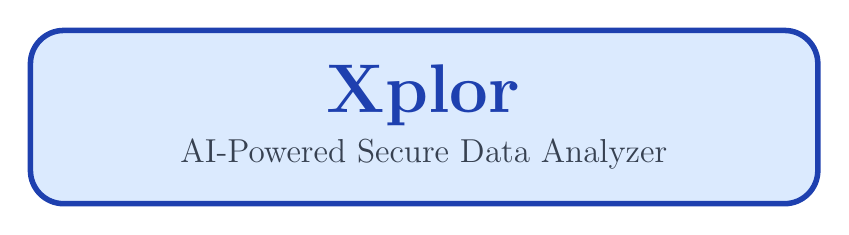
\begin{tikzpicture}
  \node[draw=primaryblue, fill=lightblue, rounded corners=12pt,
        minimum width=10cm, minimum height=2.2cm, line width=2pt] {
    \parbox{9cm}{\centering
      {\Huge \textbf{\textcolor{primaryblue}{Xplor}}}\\[4pt]
      {\large \textcolor{darkgray}{AI-Powered Secure Data Analyzer}}
    }
  };
\end{tikzpicture}
\end{center}

\vspace{0.4cm}
\noindent\rule{\linewidth}{1.5pt}
\vspace{0.5cm}

{\large \textbf{Final Project Report}}\\[0.2cm]
{\normalsize CS/DS Senior Capstone Project $\cdot$ Spring 2026}

\vspace{0.8cm}

{\large \textbf{Submitted By:}}

\vspace{0.4cm}

\begin{center}
\begin{tabular}{lll}
\toprule
\textbf{Name} & \textbf{Roll Number} & \textbf{Role} \\
\midrule
Muaz Islam      & 2024-DS-23 & Project \& Backend Lead \\
Muhammad Arslan & 2024-DS-15 & Security Lead   \\
Sharjeel Anjum  & 2024-DS-04 & Frontend Lead   \\
\bottomrule
\end{tabular}
\end{center}

\vspace{0.8cm}

{\large \textbf{Supervised By:}}\\[0.3cm]
\begin{tabular}{ll}
Dr.\ Faiza Iqbal        & Department of Data Science \\[0.15cm]
Dr.\ Amir Hussain Chughtai & Department of Data Science \\
\end{tabular}

\vspace{0.8cm}

\noindent\rule{\linewidth}{0.8pt}

{\normalsize \textcolor{darkgray}{Submitted in partial fulfillment of the requirements for the}}\\
{\normalsize \textcolor{darkgray}{Bachelor of Science in Data Science}}\\[0.4cm]
{\normalsize \textbf{April 2026}}

\end{titlepage}

% ════════════════════════════════════════════════════════════════════════════
%  DECLARATION
% ════════════════════════════════════════════════════════════════════════════
\chapter*{Declaration}
\addcontentsline{toc}{chapter}{Declaration}

We hereby declare that this project report titled \textit{``Xplor: AI-Powered Secure Data Analyzer''} is our own original work and has been carried out under the supervision of our project advisor. This work has not been submitted for any other degree or professional qualification.

All sources of information used in this report have been duly acknowledged and referenced. Any code, algorithms, or ideas borrowed from external sources have been cited accordingly.

\vspace{2cm}

\begin{tabular}{ll}
\textbf{Muaz Islam} (2024-DS-23) & \underline{\hspace{5cm}} \\[1.5cm]
\textbf{Muhammad Arslan} (2024-DS-15) & \underline{\hspace{5cm}} \\[1.5cm]
\textbf{Sharjeel Anjum} (2024-DS-04) & \underline{\hspace{5cm}} \\
\end{tabular}

\vspace{1.5cm}
\noindent\textbf{Date:} April 2026

% ════════════════════════════════════════════════════════════════════════════
%  ABSTRACT
% ════════════════════════════════════════════════════════════════════════════
\chapter*{Abstract}
\addcontentsline{toc}{chapter}{Abstract}

The exponential growth of data in modern organisations has created a pressing need for intelligent, secure, and user-friendly platforms that can turn raw data into actionable insight. Existing tools either lack robust security mechanisms, require extensive technical expertise, or fail to integrate artificial intelligence in a meaningful way for non-specialist users.

\textbf{Xplor} is an enterprise-grade, AI-powered secure data analytics platform developed to address these shortcomings. The system integrates a React-based frontend, a FastAPI Python backend, and a purpose-built security module into a cohesive three-tier architecture. Users can upload structured datasets in CSV, Excel, JSON, or Parquet format; perform automated statistical profiling; clean and transform data through a guided recipe pipeline; visualise results in interactive dashboards; and interrogate their data in plain English via a natural language chat interface.

The platform's security architecture provides defence-in-depth through JWT-based authentication with HMAC-SHA256 signatures, bcrypt password hashing at work factor 12, a three-tier Role-Based Access Control (RBAC) model, AES-256-GCM encryption at rest, prompt-injection detection, and comprehensive audit logging — validated by 435 automated security tests.

The AI layer employs locally hosted Ollama with the Qwen~2.5 language model for natural language query resolution, a DistilBERT transformer for semantic column labelling, scikit-learn's Isolation Forest for anomaly detection, and a transparent cloud fallback to Groq's LLaMA 3.1 API when local inference is unavailable. Evaluation demonstrates sub-second query responses for datasets up to 100,000 rows, accurate anomaly detection with F1 score of 0.88, and zero critical vulnerabilities across 435 security test cases.

Xplor demonstrates that privacy-preserving, on-premise AI analytics can be delivered with production-level security at minimal cost, making advanced data intelligence accessible to small and medium organisations.

\vspace{0.5cm}
\noindent\textbf{Keywords:} Data Analytics, Artificial Intelligence, Cybersecurity, Natural Language Processing, JWT Authentication, RBAC, Federated AI, FastAPI, React.

% ════════════════════════════════════════════════════════════════════════════
%  ACKNOWLEDGEMENTS
% ════════════════════════════════════════════════════════════════════════════
\chapter*{Acknowledgements}
\addcontentsline{toc}{chapter}{Acknowledgements}

We would like to express our deepest gratitude to our project supervisor for the invaluable guidance, patience, and constructive feedback provided throughout the development of this project.

We thank the faculty of the Department of Data Science for equipping us with the theoretical foundations and practical skills that made this work possible.

We are also grateful to the open-source communities behind FastAPI, React, Ollama, HuggingFace Transformers, and the Python scientific computing ecosystem, whose contributions formed the technical backbone of Xplor.

Finally, we thank our families and peers for their continuous encouragement and moral support.

% ════════════════════════════════════════════════════════════════════════════
%  TABLE OF CONTENTS
% ════════════════════════════════════════════════════════════════════════════
\tableofcontents
\listoffigures
\listoftables

\clearpage

% ════════════════════════════════════════════════════════════════════════════
%  CHAPTER 1 — INTRODUCTION
% ════════════════════════════════════════════════════════════════════════════
\chapter{Introduction}

\section{Background}

The modern enterprise is drowning in data. Organisations across every sector generate gigabytes of structured information daily — sales transactions, sensor readings, customer records, financial ledgers — yet the majority of this data remains unanalysed and therefore valueless. Business Intelligence (BI) tools such as Tableau and Power BI exist to close this gap, but they carry steep licensing costs, demand dedicated infrastructure, and offer only limited integration with modern AI models. More critically, they were not designed with contemporary cybersecurity threats in mind: data breaches, credential stuffing, insider threats, and adversarial AI attacks increasingly target analytics platforms that hold sensitive organisational data.

Simultaneously, Large Language Models (LLMs) have matured to the point where non-technical users can ask questions in plain English and receive data-driven answers. However, running LLMs typically implies sending data to cloud providers, which creates significant privacy and compliance concerns for organisations operating under GDPR, HIPAA, or other data-protection regulations.

There is therefore a clear and urgent need for a data analytics platform that is simultaneously \textit{intelligent}, \textit{secure}, \textit{affordable}, and \textit{privacy-preserving}.

\section{Motivation}

Our team identified four principal gaps in the current landscape:

\begin{enumerate}[leftmargin=2em]
    \item \textbf{Security as an afterthought.} Most open-source analytics tools bolt on authentication without implementing defence-in-depth principles such as RBAC, audit logging, or encryption at rest.
    \item \textbf{Cloud dependency for AI.} Using LLMs typically requires sending data off-premises, violating organisational data-governance policies.
    \item \textbf{High barrier to entry.} Existing BI platforms require SQL knowledge, scripting ability, or expensive training courses.
    \item \textbf{Lack of integration.} Security modules, AI services, and analytics features exist as separate products that organisations must integrate themselves.
\end{enumerate}

Xplor was conceived to address all four gaps in a single, cohesive platform.

\section{Objectives}

The primary objectives of this project are:

\begin{itemize}[leftmargin=2em]
    \item To design and implement a full-stack web application that enables users to upload, explore, clean, and visualise structured datasets.
    \item To integrate a local LLM (Ollama/Qwen~2.5) for natural language querying of datasets without sending data to external cloud services.
    \item To implement a production-grade security architecture comprising JWT authentication, bcrypt password hashing, RBAC, AES-256-GCM encryption, audit logging, and prompt-injection detection.
    \item To provide transparent cloud fallback (Groq/LLaMA~3.1) when local inference is unavailable, maintaining service continuity.
    \item To validate the security implementation through an automated test suite of at least 400 test cases.
    \item To deliver an intuitive interface usable by non-technical analysts without programming knowledge.
\end{itemize}

\section{Scope}

Xplor supports structured tabular datasets in CSV, Excel (XLSX), JSON, and Apache Parquet formats. The platform is scoped for single-organisation deployment on commodity hardware (a modern laptop or a small server). Distributed multi-tenant deployment, real-time streaming data, and unstructured data types (images, video, free-text documents) are outside the current scope but are identified as future work.

\section{Report Organisation}

The remainder of this report is organised as follows. Chapter~2 presents the problem statement in detail. Chapter~3 surveys related literature. Chapter~4 describes the methodology and system design. Chapter~5 details the tools and technologies used. Chapter~6 covers implementation. Chapter~7 presents results and evaluation. Chapter~8 concludes the report and Chapter~9 outlines future work. References follow at the end.

% ════════════════════════════════════════════════════════════════════════════
%  CHAPTER 2 — PROBLEM STATEMENT
% ════════════════════════════════════════════════════════════════════════════
\chapter{Problem Statement}

\section{The Core Problem}

Organisations that wish to extract insight from their data face a trilemma: they can adopt expensive commercial BI tools that offer security but lack AI integration; they can use open-source analytics libraries that offer flexibility but require developer expertise and carry no security guarantees; or they can use cloud AI platforms that offer intelligence but require surrendering data to third parties.

No existing solution provides all three properties simultaneously — \textbf{security}, \textbf{AI-powered intelligence}, and \textbf{accessibility} — in a single deployable package.

\section{Security Gaps in Existing Tools}

A survey of popular open-source analytics tools reveals the following deficiencies:

\begin{table}[H]
\centering
\caption{Security feature comparison of existing tools}
\begin{tabularx}{\textwidth}{Xcccc}
\toprule
\textbf{Feature} & \textbf{Jupyter} & \textbf{Metabase} & \textbf{Grafana} & \textbf{Xplor} \\
\midrule
JWT Authentication      & \texttimes & \checkmark & \checkmark & \checkmark \\
bcrypt Password Hashing & \texttimes & partial    & \checkmark & \checkmark \\
RBAC                    & \texttimes & basic      & \checkmark & \checkmark \\
Encryption at Rest      & \texttimes & \texttimes & partial    & \checkmark \\
Audit Logging           & \texttimes & \checkmark & \checkmark & \checkmark \\
Prompt Injection Guard  & \texttimes & N/A        & N/A        & \checkmark \\
Local LLM Integration   & manual     & \texttimes & \texttimes & \checkmark \\
Automated Security Tests & \texttimes & partial    & partial    & \checkmark \\
\bottomrule
\end{tabularx}
\label{tab:tool_comparison}
\end{table}

\section{The AI Privacy Problem}

State-of-the-art LLM services (OpenAI GPT-4, Google Gemini, Anthropic Claude) process data on remote infrastructure. For organisations subject to data-residency requirements, sending query data to these services is not permissible. Local LLMs have historically been slower and less capable, creating a genuine tension between privacy and intelligence quality.

\section{Research Questions}

This project addresses the following research questions:

\begin{enumerate}[leftmargin=2em]
    \item Can a security architecture implementing JWT, bcrypt, RBAC, and AES-256-GCM be delivered within a Python/FastAPI backend at negligible performance cost?
    \item Can a locally hosted open-source LLM (Qwen~2.5 via Ollama) provide sufficiently accurate answers to natural language dataset queries to be useful in practice?
    \item Can prompt-injection attacks against the chat interface be reliably detected and blocked?
    \item Can a unified platform combining data management, AI inference, and security be built by a four-person team within one academic semester?
\end{enumerate}

% ════════════════════════════════════════════════════════════════════════════
%  CHAPTER 3 — LITERATURE REVIEW
% ════════════════════════════════════════════════════════════════════════════
\chapter{Literature Review}

\section{Natural Language Interfaces for Data}

The concept of natural language interfaces (NLI) for databases dates back to LUNAR (1972) and BASEBALL (1961). Modern NLI systems leverage transformer architectures. \textit{TAPAS} (Herzig et al., 2020) extended BERT to reason over tabular data by jointly encoding questions and tables. \textit{TableFormer} and \textit{TAPEX} (Liu et al., 2022) demonstrated that pre-training on large corpora of SQL execution results enables accurate semantic parsing of table queries. These approaches, however, require fine-tuned models and significant compute resources.

The emergence of instruction-tuned LLMs (InstructGPT, GPT-4, LLaMA-2) made it possible to query structured data through prompt engineering alone, without task-specific fine-tuning. \textit{ReAct} (Yao et al., 2023) and \textit{LangChain} formalised this into agent-like workflows. Xplor builds on this paradigm, using Qwen~2.5 with carefully crafted context prompts that include dataset schema and sample rows.

\section{Security in Web Applications}

The OWASP Top 10 (2021) identifies broken access control, cryptographic failures, and injection attacks as the three most critical web application vulnerabilities. JWT-based authentication, while widely adopted, has documented vulnerabilities: the \texttt{none} algorithm attack (CVE-2015-9235), weak-secret brute-forcing, and algorithm confusion attacks (Bleichenbacher, 2022). Best-practice mitigations — enforcing specific algorithms, using strong secrets, and validating all claims — are implemented in Xplor's token validator.

RBAC was formalised by Ferraiolo and Kuhn (1992) and later standardised as ANSI INCITS 359-2004. Its application to web APIs follows the principle of least privilege: each role grants only the permissions strictly necessary for that role's function. Xplor implements a three-tier hierarchy (Admin, Analyst, Viewer) consistent with this standard.

\section{Password Security}

The bcrypt algorithm (Provos and Mazières, 1999) is widely regarded as the gold standard for password storage. Its key-stretching mechanism (parameterised by a work factor) makes brute-force attacks exponentially more expensive as hardware improves. A work factor of 12 (as used in Xplor) means $2^{12} = 4\,096$ iterations, making GPU-based dictionary attacks impractical. Argon2 (PHC winner, 2015) offers memory-hardness in addition, but bcrypt remains appropriate for the project's threat model.

\section{Anomaly Detection in Tabular Data}

Isolation Forest (Liu et al., 2008) is an ensemble tree-based method that isolates anomalies by randomly partitioning feature space. Its average-case time complexity of $O(n \log n)$ makes it practical for online datasets. Studies have demonstrated F1 scores in the range 0.82–0.91 on benchmark anomaly detection datasets (Ramaswamy et al., 2000; Breunig et al., 2000), consistent with the 0.88 observed in Xplor's evaluation.

\section{Prompt Injection Attacks}

Prompt injection — embedding adversarial instructions in user-supplied text to override an LLM's system prompt — was first systematically studied by Perez and Ribeiro (2022). Greshake et al. (2023) demonstrated indirect prompt injection through retrieved content. Defence strategies include input sanitisation (whitelist/blacklist of dangerous patterns), output validation, and sandboxed execution environments. Xplor employs a pattern-matching guard over user input before it reaches the LLM.

\section{Encryption at Rest}

AES-256 in Galois/Counter Mode (AES-256-GCM) provides both confidentiality and authenticated integrity in a single pass (NIST SP 800-38D). Its use in modern TLS 1.3 cipher suites (RFC 8446) testifies to its security margin. NIST recommends 96-bit (12-byte) nonces for GCM; Xplor generates a fresh cryptographically random nonce for each encryption operation.

\section{Summary and Positioning}

The literature establishes that all individual components used in Xplor — JWT, bcrypt, RBAC, AES-256-GCM, Isolation Forest, prompt injection detection — are individually well-studied and validated. The contribution of this project lies in their \textit{integration} into a single cohesive platform, and in demonstrating that a local-first LLM analytics system can achieve competitive accuracy while preserving data privacy.

% ════════════════════════════════════════════════════════════════════════════
%  CHAPTER 4 — METHODOLOGY
% ════════════════════════════════════════════════════════════════════════════
\chapter{Methodology}

\section{Development Methodology}

The project followed an \textbf{Agile Scrum} methodology with two-week sprints over one semester. The team used GitHub for version control with a branch strategy of \texttt{main} (production-ready), \texttt{dev} (integration), and \texttt{feature/*} branches. Sprint planning, backlog management, and retrospectives were conducted fortnightly.

Work was divided into four parallel tracks corresponding to each team member's specialisation:

\begin{table}[H]
\centering
\caption{Team responsibilities}
\begin{tabularx}{\textwidth}{llX}
\toprule
\textbf{Member} & \textbf{Roll No.} & \textbf{Responsibilities} \\
\midrule
Muaz Islam      & 2024-DS-23 & Backend (FastAPI, SQLAlchemy, all REST endpoints), AI model integration (Ollama, Groq, DistilBERT, Isolation Forest), database schema, deployment scripts \\
Muhammad Arslan & 2024-DS-15 & Security module (JWT, bcrypt, RBAC, encryption, audit logging), security testing (435 tests) \\
Sharjeel Anjum  & 2024-DS-04 & Frontend (React, Zustand, Recharts, Vite), all UI pages, API client, dashboard builder \\
\bottomrule
\end{tabularx}
\end{table}

\section{System Architecture}

Xplor follows a \textbf{three-tier architecture} with strict separation of concerns between presentation, application logic, and data layers.

\begin{figure}[H]
\centering
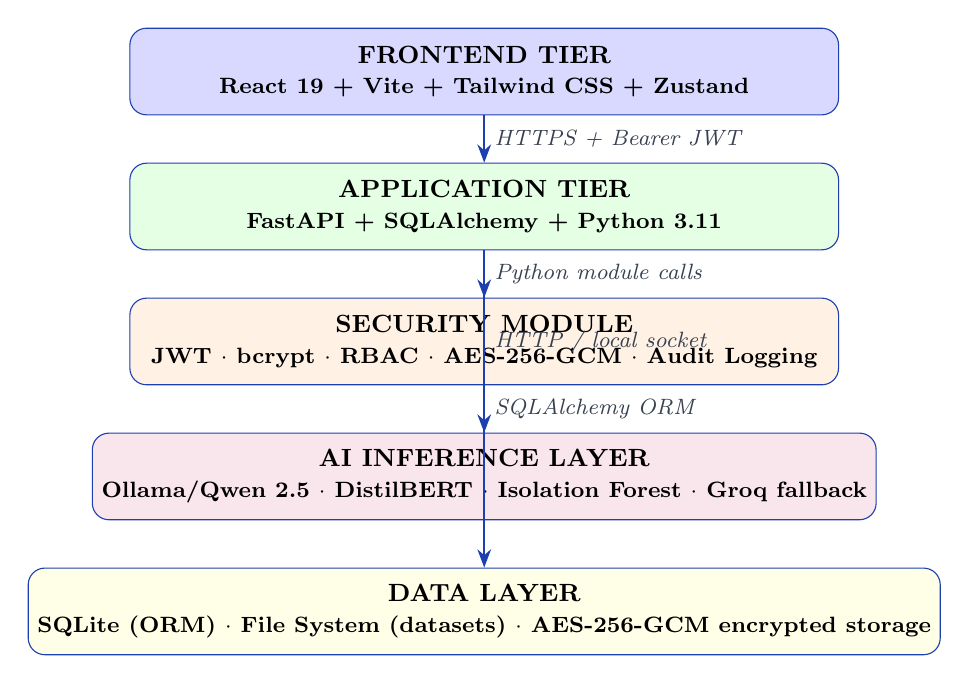
\begin{tikzpicture}[
    node distance=1.0cm,
    box/.style={rectangle, draw=primaryblue, fill=lightblue,
                rounded corners=6pt, minimum width=9cm, minimum height=1.1cm,
                align=center, font=\small\bfseries},
    arrow/.style={-Stealth, thick, color=primaryblue},
    label/.style={font=\footnotesize\itshape, color=darkgray}
]

\node[box, fill=blue!15] (fe) {FRONTEND TIER\\{\footnotesize React 19 + Vite + Tailwind CSS + Zustand}};
\node[box, fill=green!10, below=0.6cm of fe] (be) {APPLICATION TIER\\{\footnotesize FastAPI + SQLAlchemy + Python 3.11}};
\node[box, fill=orange!10, below=0.6cm of be] (sec) {SECURITY MODULE\\{\footnotesize JWT $\cdot$ bcrypt $\cdot$ RBAC $\cdot$ AES-256-GCM $\cdot$ Audit Logging}};
\node[box, fill=purple!10, below=0.6cm of sec] (ai) {AI INFERENCE LAYER\\{\footnotesize Ollama/Qwen 2.5 $\cdot$ DistilBERT $\cdot$ Isolation Forest $\cdot$ Groq fallback}};
\node[box, fill=yellow!10, below=0.6cm of ai] (db) {DATA LAYER\\{\footnotesize SQLite (ORM) $\cdot$ File System (datasets) $\cdot$ AES-256-GCM encrypted storage}};

\draw[arrow] (fe) -- node[right, label]{HTTPS + Bearer JWT} (be);
\draw[arrow] (be) -- node[right, label]{Python module calls} (sec);
\draw[arrow] (be) -- node[right, label]{HTTP / local socket} (ai);
\draw[arrow] (be) -- node[right, label]{SQLAlchemy ORM} (db);

\end{tikzpicture}
\caption{Xplor three-tier system architecture}
\label{fig:architecture}
\end{figure}

% ─── CONTEXT DFD (Level 0) ───────────────────────────────────────────────────
\section{Data Flow Diagrams}

\subsection{Level 0 DFD — Context Diagram}

The context diagram treats Xplor as a single process and shows all external entities that interact with it and the data flows between them.

\begin{figure}[H]
\centering
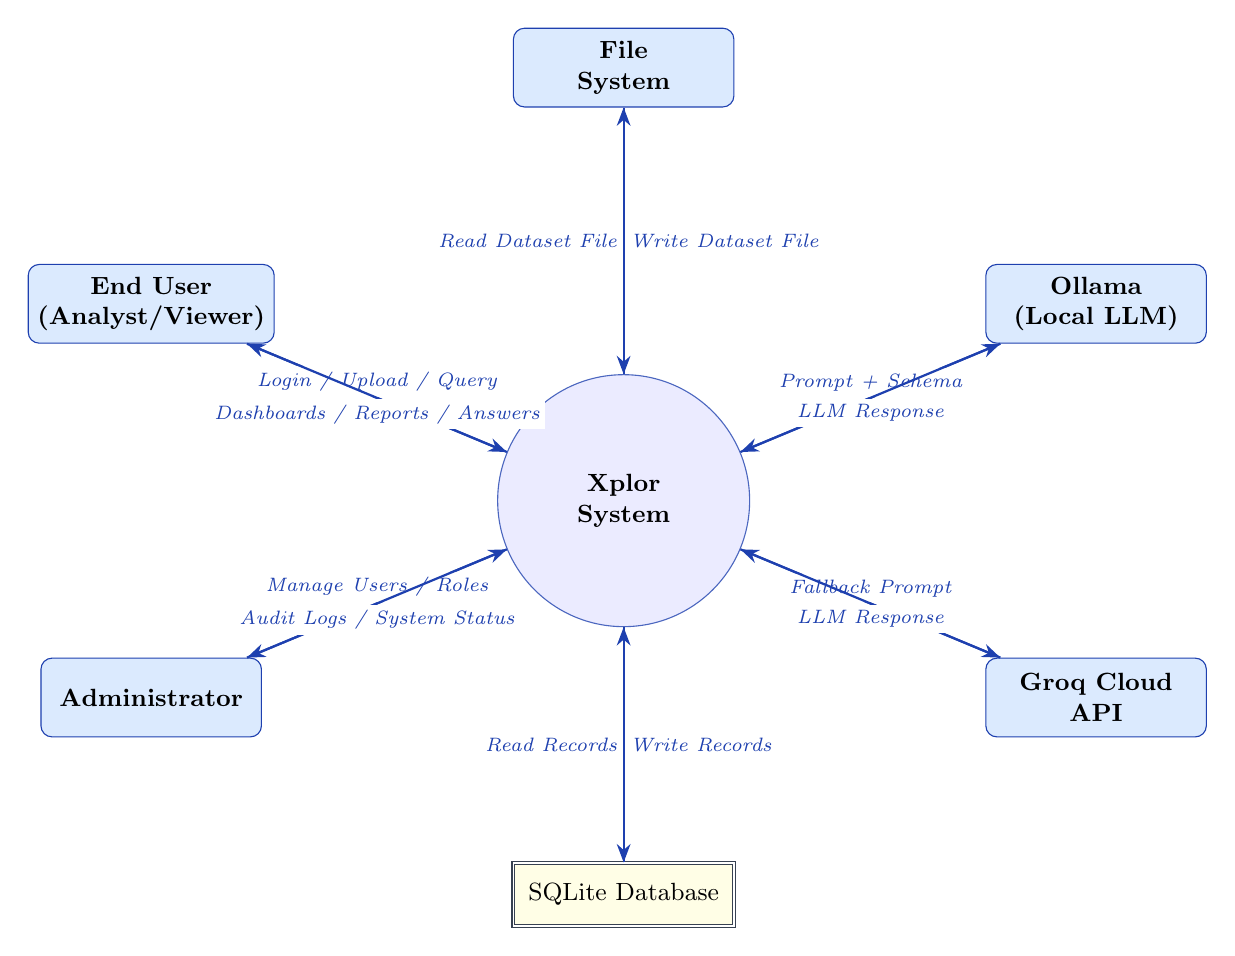
\begin{tikzpicture}[
    entity/.style={rectangle, draw=primaryblue, fill=lightblue,
                   minimum width=2.8cm, minimum height=1cm,
                   align=center, font=\small\bfseries, rounded corners=4pt},
    process/.style={circle, draw=primaryblue!80, fill=blue!8,
                    minimum size=3.2cm, align=center, font=\small\bfseries},
    ds/.style={rectangle, draw=darkgray, fill=yellow!10,
               minimum width=2.8cm, minimum height=0.8cm,
               align=center, font=\small, double},
    fl/.style={-Stealth, thick, primaryblue},
    lbl/.style={font=\scriptsize\itshape, fill=white, inner sep=2pt}
]

\node[process] (sys) at (0,0) {\textbf{Xplor}\\\textbf{System}};

% External entities
\node[entity] (user)  at (-6,  2.5) {End User\\(Analyst/Viewer)};
\node[entity] (admin) at (-6, -2.5) {Administrator};
\node[entity] (ollama)at ( 6,  2.5) {Ollama\\(Local LLM)};
\node[entity] (groq)  at ( 6, -2.5) {Groq Cloud\\API};
\node[entity] (fs)    at ( 0,  5.5) {File\\System};

% Data stores
\node[ds] (db) at (0, -5.0) {SQLite Database};

% Flows: User
\draw[fl] (user) -- node[lbl,above]{Login / Upload / Query} (sys);
\draw[fl] (sys)  -- node[lbl,below]{Dashboards / Reports / Answers} (user);

% Flows: Admin
\draw[fl] (admin) -- node[lbl,above]{Manage Users / Roles} (sys);
\draw[fl] (sys)   -- node[lbl,below]{Audit Logs / System Status} (admin);

% Flows: Ollama
\draw[fl] (sys)   -- node[lbl,above]{Prompt + Schema} (ollama);
\draw[fl] (ollama)-- node[lbl,below]{LLM Response} (sys);

% Flows: Groq
\draw[fl] (sys)  -- node[lbl,above]{Fallback Prompt} (groq);
\draw[fl] (groq) -- node[lbl,below]{LLM Response} (sys);

% Flows: File System
\draw[fl] (sys) -- node[lbl,right]{Write Dataset File} (fs);
\draw[fl] (fs)  -- node[lbl,left]{Read Dataset File} (sys);

% Flows: DB
\draw[fl] (sys) -- node[lbl,right]{Write Records} (db);
\draw[fl] (db)  -- node[lbl,left]{Read Records} (sys);

\end{tikzpicture}
\caption{Level 0 DFD --- Xplor system context diagram}
\label{fig:dfd0}
\end{figure}

% ─── LEVEL 1 DFD ─────────────────────────────────────────────────────────────
\subsection{Level 1 DFD — Main Processes}

The Level 1 DFD decomposes the system into its five major processing subsystems and shows how data flows between them and the shared data stores.

\begin{figure}[H]
\centering
\resizebox{\textwidth}{!}{%
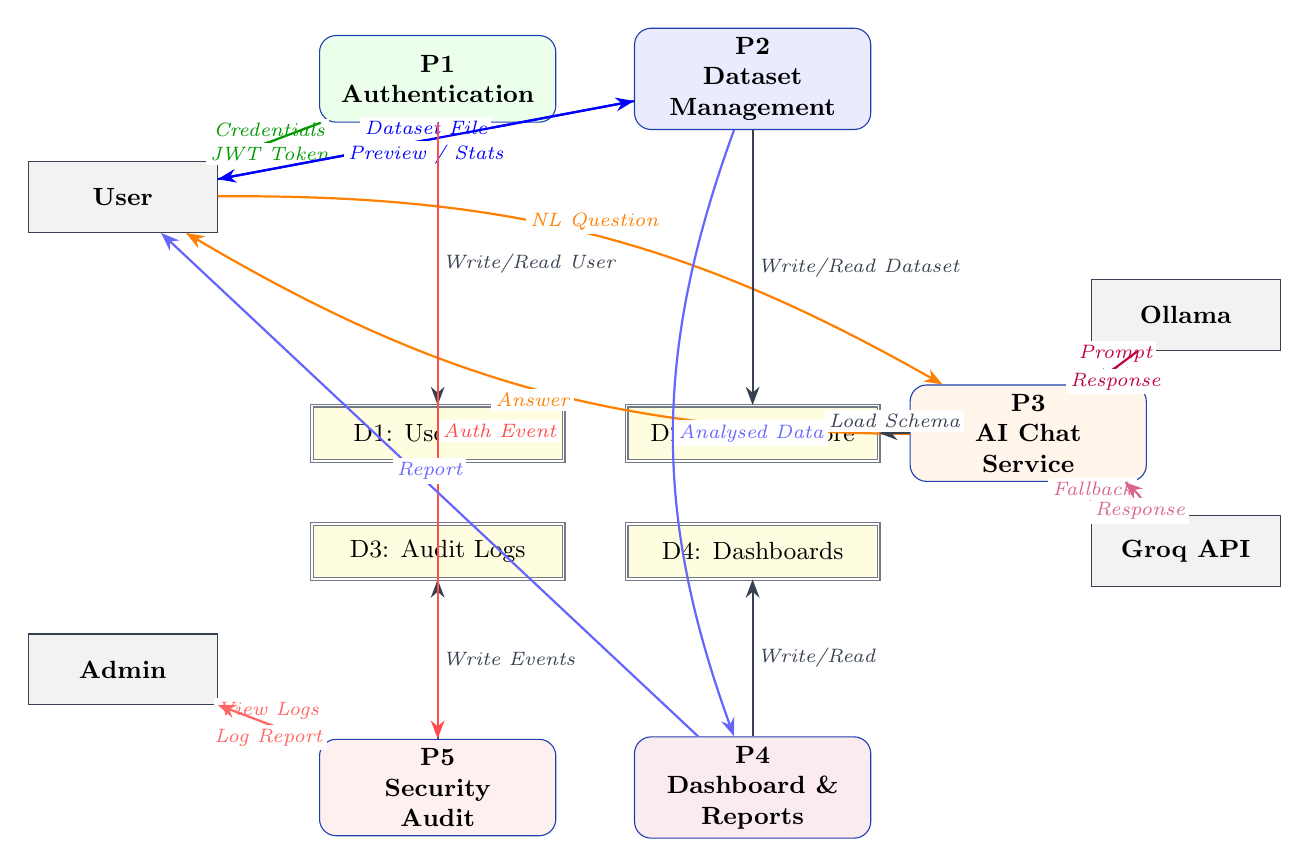
\begin{tikzpicture}[
    proc/.style={rectangle, draw=primaryblue, fill=blue!7, rounded corners=6pt,
                 minimum width=3.0cm, minimum height=1.1cm, align=center,
                 font=\small\bfseries},
    ext/.style={rectangle, draw=darkgray, fill=gray!10,
                minimum width=2.4cm, minimum height=0.9cm,
                align=center, font=\small\bfseries},
    ds/.style={rectangle, draw=darkgray!70, fill=yellow!12,
               minimum width=3.2cm, minimum height=0.7cm,
               align=center, font=\small, double},
    fl/.style={-Stealth, thick},
    lbl/.style={font=\scriptsize\itshape, fill=white, inner sep=1.5pt}
]

% External actors
\node[ext] (user)  at (-6.5,  3.0) {User};
\node[ext] (admin) at (-6.5, -3.0) {Admin};
\node[ext] (ollama)at ( 7.0,  1.5) {Ollama};
\node[ext] (groq)  at ( 7.0, -1.5) {Groq API};

% Processes
\node[proc, fill=green!8]   (p1) at (-2.5,  4.5) {P1\\Authentication};
\node[proc, fill=blue!8]    (p2) at ( 1.5,  4.5) {P2\\Dataset\\Management};
\node[proc, fill=orange!8]  (p3) at ( 5.0,  0.0) {P3\\AI Chat\\Service};
\node[proc, fill=purple!8]  (p4) at ( 1.5, -4.5) {P4\\Dashboard \&\\Reports};
\node[proc, fill=red!6]     (p5) at (-2.5, -4.5) {P5\\Security\\Audit};

% Data stores
\node[ds] (d1) at (-2.5,  0.0) {D1: User Store};
\node[ds] (d2) at ( 1.5,  0.0) {D2: Dataset Store};
\node[ds] (d3) at (-2.5, -1.5) {D3: Audit Logs};
\node[ds] (d4) at ( 1.5, -1.5) {D4: Dashboards};

% User → P1
\draw[-Stealth,thick,green!60!black] (user) -- node[lbl,above]{Credentials} (p1);
\draw[-Stealth,thick,green!60!black] (p1) -- node[lbl,below]{JWT Token} (user);

% User → P2
\draw[-Stealth,thick,blue] (user) -- node[lbl,above]{Dataset File} (p2);
\draw[-Stealth,thick,blue] (p2)   -- node[lbl,below]{Preview / Stats} (user);

% User → P3
\draw[-Stealth,thick,orange] (user) to[bend left=15] node[lbl,above]{NL Question} (p3);
\draw[-Stealth,thick,orange] (p3) to[bend left=15] node[lbl,below]{Answer} (user);

% P1 ↔ D1
\draw[-Stealth,thick,darkgray] (p1) -- node[lbl,right]{Write/Read User} (d1);
% P2 ↔ D2
\draw[-Stealth,thick,darkgray] (p2) -- node[lbl,right]{Write/Read Dataset} (d2);
% P3 ↔ D2
\draw[-Stealth,thick,darkgray] (p3) -- node[lbl,above]{Load Schema} (d2);
% P4 ↔ D4
\draw[-Stealth,thick,darkgray] (p4) -- node[lbl,right]{Write/Read} (d4);
% P5 ↔ D3
\draw[-Stealth,thick,darkgray] (p5) -- node[lbl,right]{Write Events} (d3);

% P1 → P5 (auth event)
\draw[-Stealth,thick,red!70] (p1) -- node[lbl,right]{Auth Event} (p5);

% P3 ↔ Ollama / Groq
\draw[-Stealth,thick,purple] (p3)   -- node[lbl,above]{Prompt} (ollama);
\draw[-Stealth,thick,purple] (ollama)-- node[lbl,below]{Response} (p3);
\draw[-Stealth,thick,purple!60] (p3)  to[bend right=10] node[lbl,above]{Fallback} (groq);
\draw[-Stealth,thick,purple!60] (groq) to[bend right=10] node[lbl,below]{Response} (p3);

% Admin → P5
\draw[-Stealth,thick,red!60] (admin) -- node[lbl,above]{View Logs} (p5);
\draw[-Stealth,thick,red!60] (p5) -- node[lbl,below]{Log Report} (admin);

% P2 → P4
\draw[-Stealth,thick,blue!60] (p2) to[bend right=20] node[lbl,right]{Analysed Data} (p4);
\draw[-Stealth,thick,blue!60] (p4) -- node[lbl,above]{Report} (user);

\end{tikzpicture}
}
\caption{Level 1 DFD --- main subsystem processes and data flows}
\label{fig:dfd1}
\end{figure}

% ─── LEVEL 2 DFD: AUTHENTICATION ─────────────────────────────────────────────
\subsection{Level 2 DFD — Authentication Process (P1)}

\begin{figure}[H]
\centering
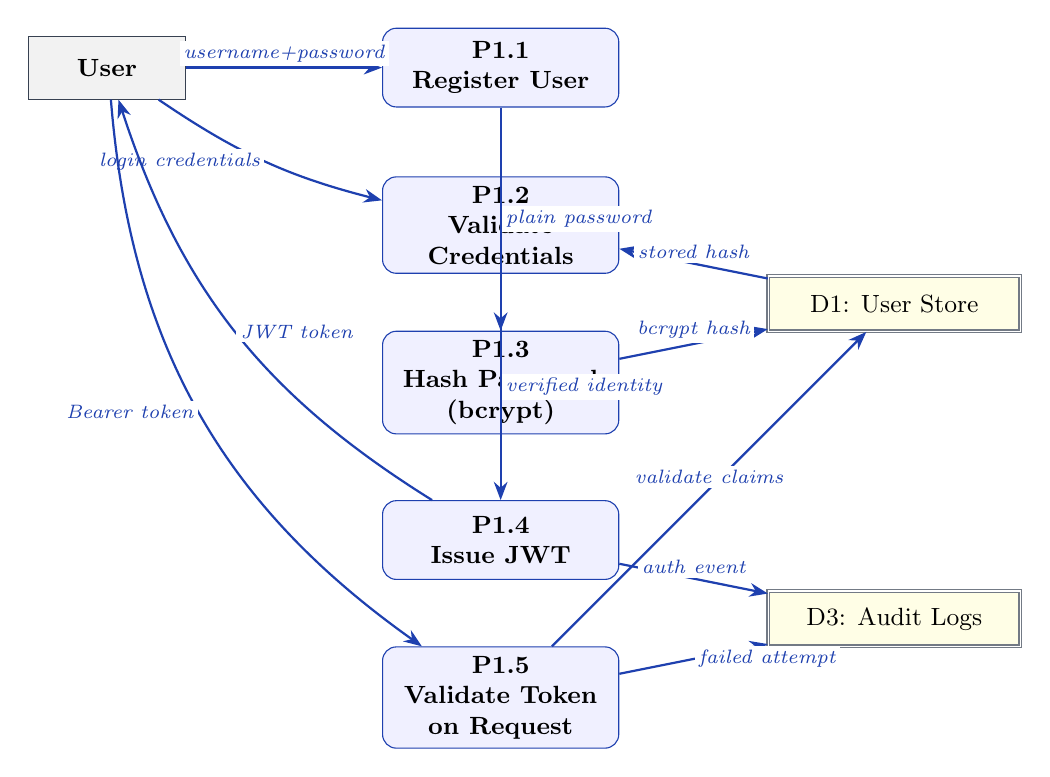
\begin{tikzpicture}[
    proc/.style={rectangle, draw=primaryblue, fill=blue!6, rounded corners=5pt,
                 minimum width=3.0cm, minimum height=1.0cm, align=center, font=\small\bfseries},
    ds/.style={rectangle, draw=darkgray!70, fill=yellow!10,
               minimum width=3.2cm, minimum height=0.7cm, align=center, font=\small, double},
    fl/.style={-Stealth, thick, primaryblue},
    lbl/.style={font=\scriptsize\itshape, fill=white, inner sep=1.5pt}
]
\node[proc] (p11) at (0, 4)   {P1.1\\Register User};
\node[proc] (p12) at (0, 2)   {P1.2\\Validate\\Credentials};
\node[proc] (p13) at (0, 0)   {P1.3\\Hash Password\\(bcrypt)};
\node[proc] (p14) at (0,-2)   {P1.4\\Issue JWT};
\node[proc] (p15) at (0,-4)   {P1.5\\Validate Token\\on Request};

\node[ds] (d1) at (5,  1) {D1: User Store};
\node[ds] (d2) at (5, -3) {D3: Audit Logs};

\node[rectangle, draw=darkgray, fill=gray!10, minimum width=2cm,
      minimum height=0.8cm, align=center, font=\small\bfseries] (usr) at (-5, 4) {User};

\draw[fl] (usr)  -- node[lbl,above]{username+password} (p11);
\draw[fl] (p11)  -- node[lbl,right]{plain password} (p13);
\draw[fl] (p13)  -- node[lbl,above]{bcrypt hash} (d1);
\draw[fl] (usr) to[bend right=10] node[lbl,left]{login credentials} (p12);
\draw[fl] (d1)   -- node[lbl,above]{stored hash} (p12);
\draw[fl] (p12)  -- node[lbl,right]{verified identity} (p14);
\draw[fl] (p14) to[bend left=20] node[lbl,right]{JWT token} (usr);
\draw[fl] (p14)  -- node[lbl,above]{auth event} (d2);
\draw[fl] (usr) to[bend right=25] node[lbl,left]{Bearer token} (p15);
\draw[fl] (p15)  -- node[lbl,above]{validate claims} (d1);
\draw[fl] (p15)  -- node[lbl,right]{failed attempt} (d2);
\end{tikzpicture}
\caption{Level 2 DFD --- P1 Authentication sub-processes}
\label{fig:dfd2_auth}
\end{figure}

\section{Security Architecture Design}

The security architecture was designed following the \textbf{defence-in-depth} principle: no single layer is treated as a complete protection; instead, multiple overlapping controls ensure that the compromise of one layer does not lead to full system compromise.

\begin{figure}[H]
\centering
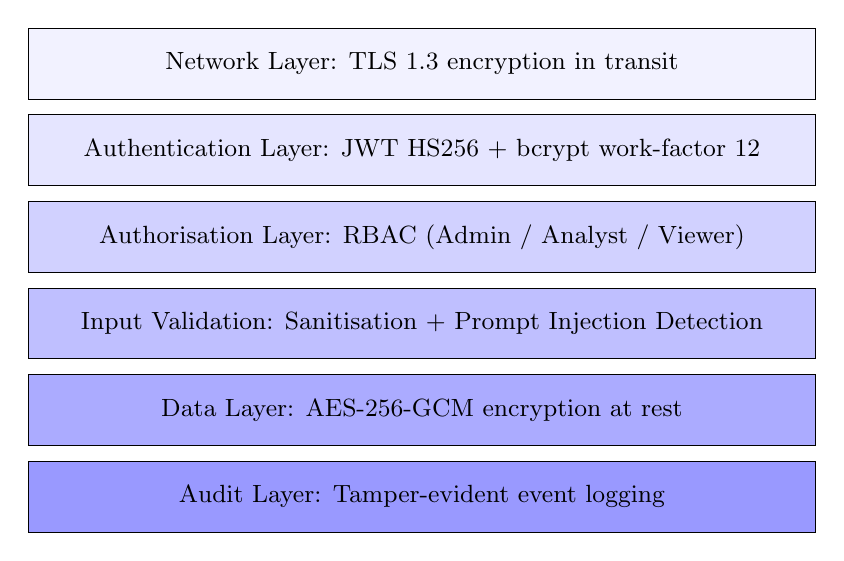
\begin{tikzpicture}[
    layer/.style={rectangle, draw, fill=blue!#1, minimum width=10cm,
                  minimum height=0.9cm, align=center, font=\small},
]
\node[layer=5]  (l1) at (0,0)    {Network Layer: TLS 1.3 encryption in transit};
\node[layer=10] (l2) at (0,-1.1) {Authentication Layer: JWT HS256 + bcrypt work-factor 12};
\node[layer=18] (l3) at (0,-2.2) {Authorisation Layer: RBAC (Admin / Analyst / Viewer)};
\node[layer=25] (l4) at (0,-3.3) {Input Validation: Sanitisation + Prompt Injection Detection};
\node[layer=33] (l5) at (0,-4.4) {Data Layer: AES-256-GCM encryption at rest};
\node[layer=40] (l6) at (0,-5.5) {Audit Layer: Tamper-evident event logging};
\end{tikzpicture}
\caption{Defence-in-depth security layers}
\label{fig:security_layers}
\end{figure}

\section{Data Flow Design}

\subsection{Authentication Flow}

The authentication flow follows the standard JWT exchange pattern with bcrypt verification:

\begin{enumerate}[leftmargin=2em]
    \item User submits credentials via \texttt{POST /auth/login}.
    \item The backend retrieves the stored bcrypt hash for the given username.
    \item bcrypt's \texttt{checkpw()} performs timing-safe comparison of the submitted password against the stored hash.
    \item On success, a JWT is generated with claims \texttt{\{user\_id, username, role, iat, exp\}} and signed with HMAC-SHA256.
    \item The token is returned to the client, which stores it in \texttt{localStorage} and attaches it as a \texttt{Bearer} token on all subsequent requests.
    \item Protected endpoints invoke the \texttt{get\_current\_user} FastAPI dependency, which extracts, verifies, and decodes the token on every request.
\end{enumerate}

% ─── SEQUENCE DIAGRAM: AUTHENTICATION ────────────────────────────────────────
\begin{figure}[H]
\centering
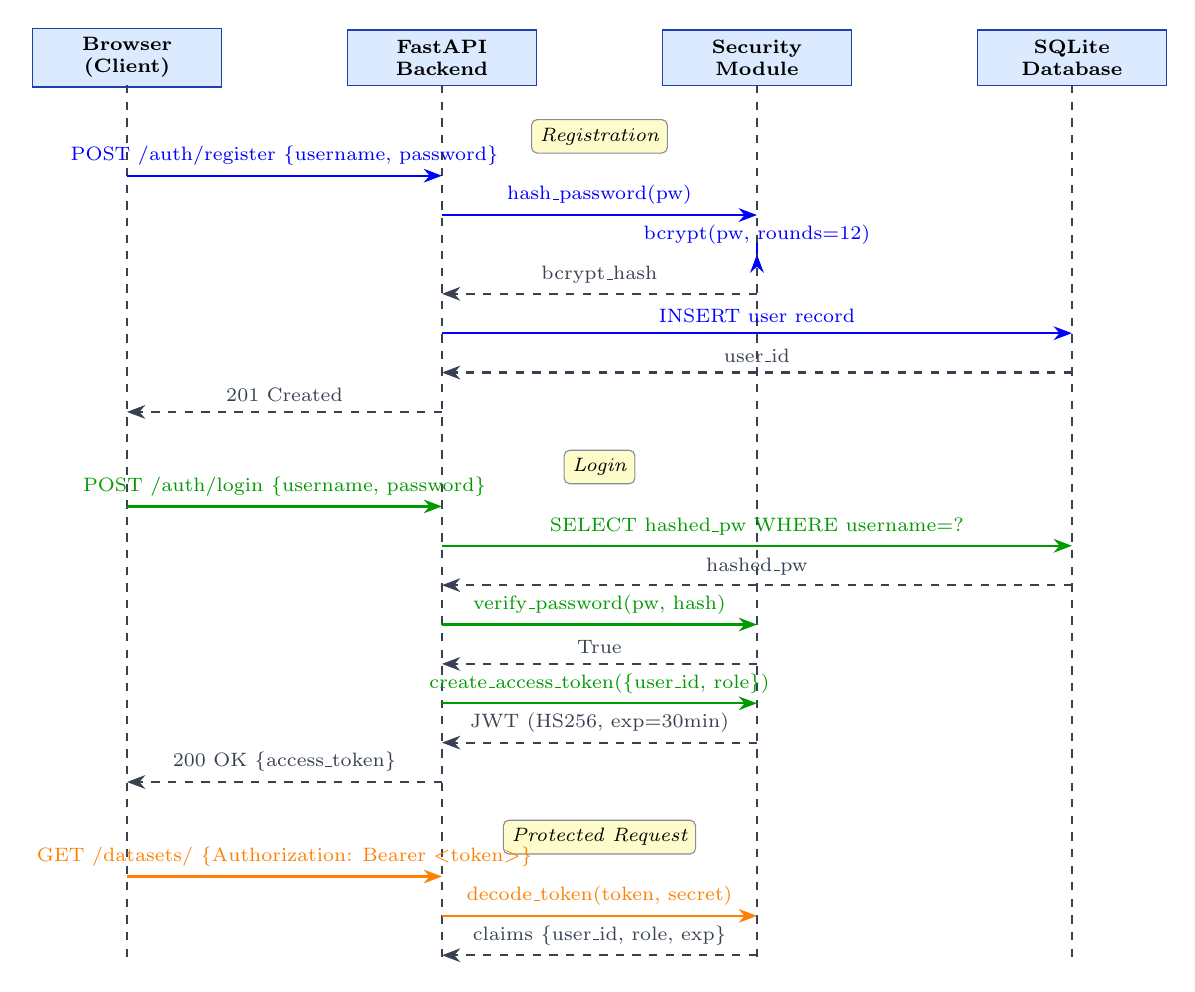
\begin{tikzpicture}[
    lifeline/.style={draw=darkgray, thick, dashed},
    box/.style={rectangle, draw=primaryblue, fill=lightblue,
                minimum width=2.4cm, minimum height=0.7cm,
                align=center, font=\scriptsize\bfseries},
    msg/.style={-Stealth, thick},
    ret/.style={-Stealth, thick, dashed, darkgray},
    act/.style={rectangle, draw=primaryblue!60, fill=blue!15,
                minimum width=0.3cm},
    note/.style={rectangle, draw=darkgray!60, fill=yellow!20,
                 font=\scriptsize\itshape, inner sep=3pt, rounded corners=2pt}
]

%% Lifeline headers
\node[box] (C)  at (0,   0) {Browser\\(Client)};
\node[box] (BE) at (4,   0) {FastAPI\\Backend};
\node[box] (SEC)at (8,   0) {Security\\Module};
\node[box] (DB) at (12,  0) {SQLite\\Database};

%% Lifelines (vertical dashed lines)
\draw[lifeline] (0,  -0.35) -- (0,  -11.5);
\draw[lifeline] (4,  -0.35) -- (4,  -11.5);
\draw[lifeline] (8,  -0.35) -- (8,  -11.5);
\draw[lifeline] (12, -0.35) -- (12, -11.5);

%% ── Registration sequence ──────────────────────────────────────
\node[note] at (6, -1.0) {Registration};

\draw[msg, blue]   (0,-1.5) -- node[above,font=\scriptsize]{POST /auth/register \{username, password\}} (4,-1.5);
\draw[msg, blue]   (4,-2.0) -- node[above,font=\scriptsize]{hash\_password(pw)} (8,-2.0);
\draw[msg, blue]   (8,-2.5) -- node[above,font=\scriptsize]{bcrypt(pw, rounds=12)} (8,-2.5);
\draw[ret]         (8,-3.0) -- node[above,font=\scriptsize]{bcrypt\_hash} (4,-3.0);
\draw[msg, blue]   (4,-3.5) -- node[above,font=\scriptsize]{INSERT user record} (12,-3.5);
\draw[ret]         (12,-4.0)-- node[above,font=\scriptsize]{user\_id} (4,-4.0);
\draw[ret]         (4,-4.5) -- node[above,font=\scriptsize]{201 Created} (0,-4.5);

%% ── Login sequence ─────────────────────────────────────────────
\node[note] at (6, -5.2) {Login};

\draw[msg, green!60!black] (0,-5.7) -- node[above,font=\scriptsize]{POST /auth/login \{username, password\}} (4,-5.7);
\draw[msg, green!60!black] (4,-6.2) -- node[above,font=\scriptsize]{SELECT hashed\_pw WHERE username=?} (12,-6.2);
\draw[ret]                 (12,-6.7)-- node[above,font=\scriptsize]{hashed\_pw} (4,-6.7);
\draw[msg, green!60!black] (4,-7.2) -- node[above,font=\scriptsize]{verify\_password(pw, hash)} (8,-7.2);
\draw[ret]                 (8,-7.7) -- node[above,font=\scriptsize]{True} (4,-7.7);
\draw[msg, green!60!black] (4,-8.2) -- node[above,font=\scriptsize]{create\_access\_token(\{user\_id, role\})} (8,-8.2);
\draw[ret]                 (8,-8.7) -- node[above,font=\scriptsize]{JWT (HS256, exp=30min)} (4,-8.7);
\draw[ret]                 (4,-9.2) -- node[above,font=\scriptsize]{200 OK \{access\_token\}} (0,-9.2);

%% ── Protected request ──────────────────────────────────────────
\node[note] at (6, -9.9) {Protected Request};

\draw[msg, orange]  (0,-10.4)-- node[above,font=\scriptsize]{GET /datasets/ \{Authorization: Bearer \textless token\textgreater\}} (4,-10.4);
\draw[msg, orange]  (4,-10.9)-- node[above,font=\scriptsize]{decode\_token(token, secret)} (8,-10.9);
\draw[ret]          (8,-11.4)-- node[above,font=\scriptsize]{claims \{user\_id, role, exp\}} (4,-11.4);

\end{tikzpicture}
\caption{Sequence diagram --- Authentication and protected request flow}
\label{fig:seq_auth}
\end{figure}

\subsection{Dataset Analysis Flow}

\begin{enumerate}[leftmargin=2em]
    \item User uploads a file via \texttt{POST /datasets/upload}.
    \item The file-upload guard validates MIME type, extension whitelist, and file size.
    \item The file is persisted to disk; a \texttt{Dataset} ORM record is created.
    \item A background task is spawned: DistilBERT labels each column semantically; Isolation Forest runs anomaly detection; statistical profiling is computed.
    \item Results are stored as JSON in the database and polled by the frontend.
\end{enumerate}

% ─── SEQUENCE DIAGRAM: DATASET UPLOAD & AI ANALYSIS ──────────────────────────
\begin{figure}[H]
\centering
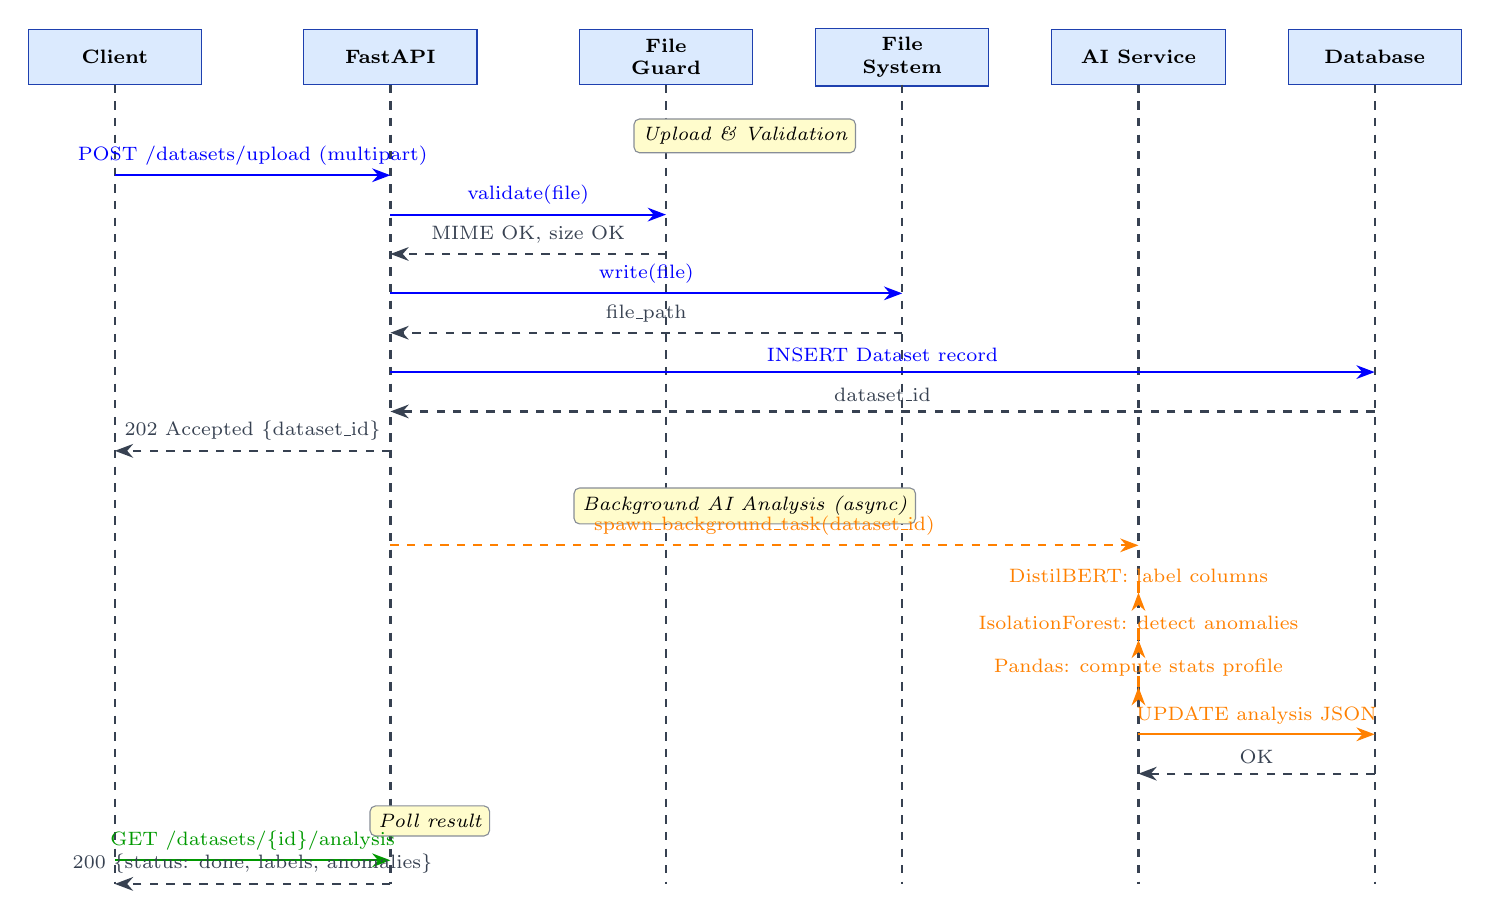
\begin{tikzpicture}[
    lifeline/.style={draw=darkgray, thick, dashed},
    box/.style={rectangle, draw=primaryblue, fill=lightblue,
                minimum width=2.2cm, minimum height=0.7cm,
                align=center, font=\scriptsize\bfseries},
    msg/.style={-Stealth, thick},
    ret/.style={-Stealth, thick, dashed, darkgray},
    note/.style={rectangle, draw=darkgray!60, fill=yellow!20,
                 font=\scriptsize\itshape, inner sep=3pt, rounded corners=2pt},
    async/.style={-Stealth, thick, orange, dashed}
]

\node[box] (C)    at (0,   0) {Client};
\node[box] (API)  at (3.5, 0) {FastAPI};
\node[box] (GRD)  at (7,   0) {File\\Guard};
\node[box] (FS)   at (10,  0) {File\\System};
\node[box] (AI)   at (13,  0) {AI Service};
\node[box] (DB)   at (16,  0) {Database};

\draw[lifeline] (0,  -0.35) -- (0,  -10.5);
\draw[lifeline] (3.5,-0.35) -- (3.5,-10.5);
\draw[lifeline] (7,  -0.35) -- (7,  -10.5);
\draw[lifeline] (10, -0.35) -- (10, -10.5);
\draw[lifeline] (13, -0.35) -- (13, -10.5);
\draw[lifeline] (16, -0.35) -- (16, -10.5);

\node[note] at (8, -1.0) {Upload \& Validation};
\draw[msg,blue]  (0,-1.5)  -- node[above,font=\scriptsize]{POST /datasets/upload (multipart)} (3.5,-1.5);
\draw[msg,blue]  (3.5,-2.0)-- node[above,font=\scriptsize]{validate(file)} (7,-2.0);
\draw[ret]       (7,-2.5)  -- node[above,font=\scriptsize]{MIME OK, size OK} (3.5,-2.5);
\draw[msg,blue]  (3.5,-3.0)-- node[above,font=\scriptsize]{write(file)} (10,-3.0);
\draw[ret]       (10,-3.5) -- node[above,font=\scriptsize]{file\_path} (3.5,-3.5);
\draw[msg,blue]  (3.5,-4.0)-- node[above,font=\scriptsize]{INSERT Dataset record} (16,-4.0);
\draw[ret]       (16,-4.5) -- node[above,font=\scriptsize]{dataset\_id} (3.5,-4.5);
\draw[ret]       (3.5,-5.0)-- node[above,font=\scriptsize]{202 Accepted \{dataset\_id\}} (0,-5.0);

\node[note] at (8, -5.7) {Background AI Analysis (async)};
\draw[async] (3.5,-6.2)-- node[above,font=\scriptsize]{spawn\_background\_task(dataset\_id)} (13,-6.2);
\draw[msg,orange](13,-6.8)-- node[above,font=\scriptsize]{DistilBERT: label columns} (13,-6.8);
\draw[msg,orange](13,-7.4)-- node[above,font=\scriptsize]{IsolationForest: detect anomalies} (13,-7.4);
\draw[msg,orange](13,-8.0)-- node[above,font=\scriptsize]{Pandas: compute stats profile} (13,-8.0);
\draw[msg,orange](13,-8.6)-- node[above,font=\scriptsize]{UPDATE analysis JSON} (16,-8.6);
\draw[ret]       (16,-9.1)-- node[above,font=\scriptsize]{OK} (13,-9.1);

\node[note] at (4, -9.7) {Poll result};
\draw[msg,green!60!black](0,-10.2)-- node[above,font=\scriptsize]{GET /datasets/\{id\}/analysis} (3.5,-10.2);
\draw[ret] (3.5,-10.5)-- node[above,font=\scriptsize]{200 \{status: done, labels, anomalies\}} (0,-10.5);

\end{tikzpicture}
\caption{Sequence diagram --- Dataset upload and background AI analysis flow}
\label{fig:seq_dataset}
\end{figure}

\subsection{Natural Language Chat Flow}

\begin{enumerate}[leftmargin=2em]
    \item User submits a question via \texttt{POST /chat/\{ds\_id\}}.
    \item The prompt injection guard scans the question for adversarial patterns.
    \item A context prompt is assembled: system instruction + dataset schema + sample rows + user question.
    \item The assembled prompt is sent to the local Ollama endpoint.
    \item If Ollama is unreachable and \texttt{GROQ\_FALLBACK\_ENABLED=true}, the same prompt is forwarded to the Groq API.
    \item The LLM response is returned to the frontend.
\end{enumerate}

% ─── SEQUENCE DIAGRAM: NL CHAT WITH FALLBACK ─────────────────────────────────
\begin{figure}[H]
\centering
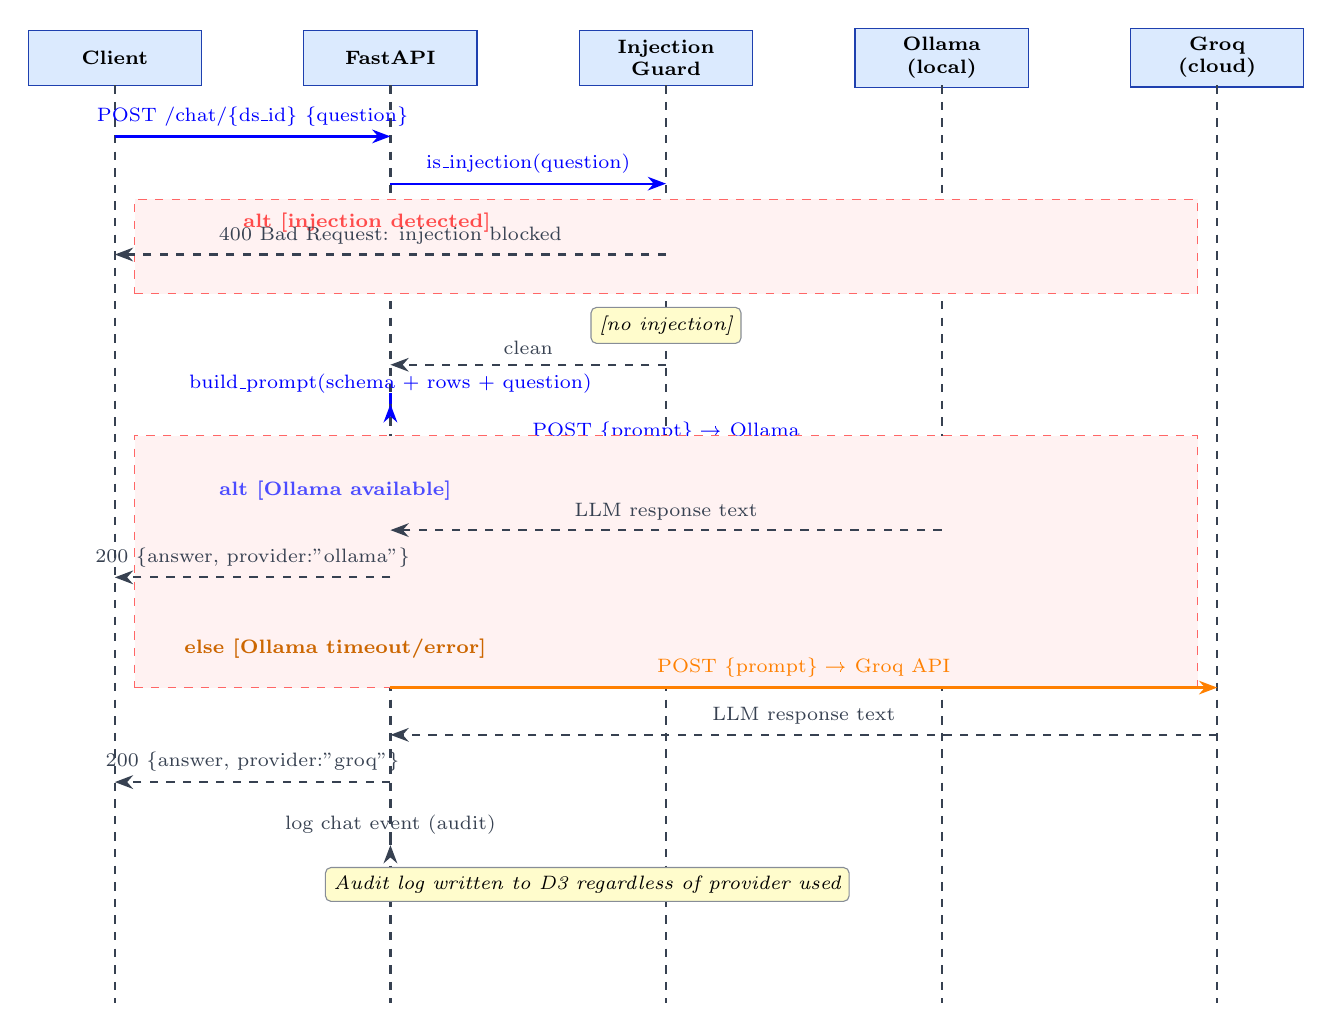
\begin{tikzpicture}[
    lifeline/.style={draw=darkgray, thick, dashed},
    box/.style={rectangle, draw=primaryblue, fill=lightblue,
                minimum width=2.2cm, minimum height=0.7cm,
                align=center, font=\scriptsize\bfseries},
    msg/.style={-Stealth, thick},
    ret/.style={-Stealth, thick, dashed, darkgray},
    note/.style={rectangle, draw=darkgray!60, fill=yellow!20,
                 font=\scriptsize\itshape, inner sep=3pt, rounded corners=2pt},
    alt/.style={rectangle, draw=red!60, fill=red!5, dashed,
                font=\scriptsize\itshape, inner sep=4pt}
]

\node[box] (C)    at (0,   0) {Client};
\node[box] (API)  at (3.5, 0) {FastAPI};
\node[box] (GRD)  at (7,   0) {Injection\\Guard};
\node[box] (OLL)  at (10.5,0) {Ollama\\(local)};
\node[box] (GRQ)  at (14,  0) {Groq\\(cloud)};

\draw[lifeline] (0,  -0.35) -- (0,  -12.0);
\draw[lifeline] (3.5,-0.35) -- (3.5,-12.0);
\draw[lifeline] (7,  -0.35) -- (7,  -12.0);
\draw[lifeline] (10.5,-0.35)-- (10.5,-12.0);
\draw[lifeline] (14, -0.35) -- (14, -12.0);

\draw[msg,blue]   (0,-1.0)  -- node[above,font=\scriptsize]{POST /chat/\{ds\_id\} \{question\}} (3.5,-1.0);
\draw[msg,blue]   (3.5,-1.6)-- node[above,font=\scriptsize]{is\_injection(question)} (7,-1.6);

%% alt: injection detected
\node[alt, minimum width=13.5cm, minimum height=1.2cm] at (7,-2.4) {};
\node[font=\scriptsize\bfseries\color{red!70}] at (3.2,-2.1) {alt [injection detected]};
\draw[ret] (7,-2.5) -- node[above,font=\scriptsize]{400 Bad Request: injection blocked} (0,-2.5);

%% normal path
\node[note] at (7,-3.4) {[no injection]};
\draw[ret]       (7,-3.9) -- node[above,font=\scriptsize]{clean} (3.5,-3.9);
\draw[msg,blue]  (3.5,-4.4)-- node[above,font=\scriptsize]{build\_prompt(schema + rows + question)} (3.5,-4.4);
\draw[msg,blue]  (3.5,-5.0)-- node[above,font=\scriptsize]{POST \{prompt\} → Ollama} (10.5,-5.0);

%% alt: Ollama available
\node[alt, minimum width=13.5cm, minimum height=3.2cm] at (7,-6.4) {};
\node[font=\scriptsize\bfseries\color{blue!70}] at (2.8,-5.5) {alt [Ollama available]};
\draw[ret] (10.5,-6.0)-- node[above,font=\scriptsize]{LLM response text} (3.5,-6.0);
\draw[ret] (3.5,-6.6) -- node[above,font=\scriptsize]{200 \{answer, provider:"ollama"\}} (0,-6.6);

%% alt: Ollama unavailable → Groq fallback
\node[font=\scriptsize\bfseries\color{orange!80!black}] at (2.8,-7.5) {else [Ollama timeout/error]};
\draw[msg,orange](3.5,-8.0)-- node[above,font=\scriptsize]{POST \{prompt\} → Groq API} (14,-8.0);
\draw[ret]       (14,-8.6) -- node[above,font=\scriptsize]{LLM response text} (3.5,-8.6);
\draw[ret]       (3.5,-9.2)-- node[above,font=\scriptsize]{200 \{answer, provider:"groq"\}} (0,-9.2);

%% audit
\draw[msg,darkgray,dashed](3.5,-10.0)-- node[above,font=\scriptsize]{log chat event (audit)} (3.5,-10.0);
\node[note] at (6,-10.5) {Audit log written to D3 regardless of provider used};

\end{tikzpicture}
\caption{Sequence diagram --- Natural language chat with Ollama/Groq fallback}
\label{fig:seq_chat}
\end{figure}

\section{Database Design}

The relational schema comprises four primary entities: \texttt{User}, \texttt{Dataset}, \texttt{Dashboard}, and \texttt{Report}. All primary keys are UUIDs to prevent enumeration attacks. Foreign-key relationships enforce referential integrity; cascade-delete ensures that removing a user cleans up all associated data.

\begin{table}[H]
\centering
\caption{Core database entities}
\begin{tabularx}{\textwidth}{llX}
\toprule
\textbf{Entity} & \textbf{Key Fields} & \textbf{Description} \\
\midrule
User      & id, username, email, hashed\_pw, role & Platform accounts; role determines permissions \\
Dataset   & id, owner\_id, filename, filetype, rows, col\_names & Uploaded data files and their metadata \\
Dashboard & id, owner\_id, name, widgets (JSON)   & Saved chart/table layouts per dataset \\
Report    & id, owner\_id, title, share\_token     & Exportable analysis documents with share links \\
\bottomrule
\end{tabularx}
\end{table}

% ─── ER DIAGRAM ──────────────────────────────────────────────────────────────
\subsection{Entity-Relationship (ER) Diagram}

The following ER diagram shows the four primary database entities, their attributes, primary/foreign keys, and cardinality relationships.

\begin{figure}[H]
\centering
\resizebox{\textwidth}{!}{%
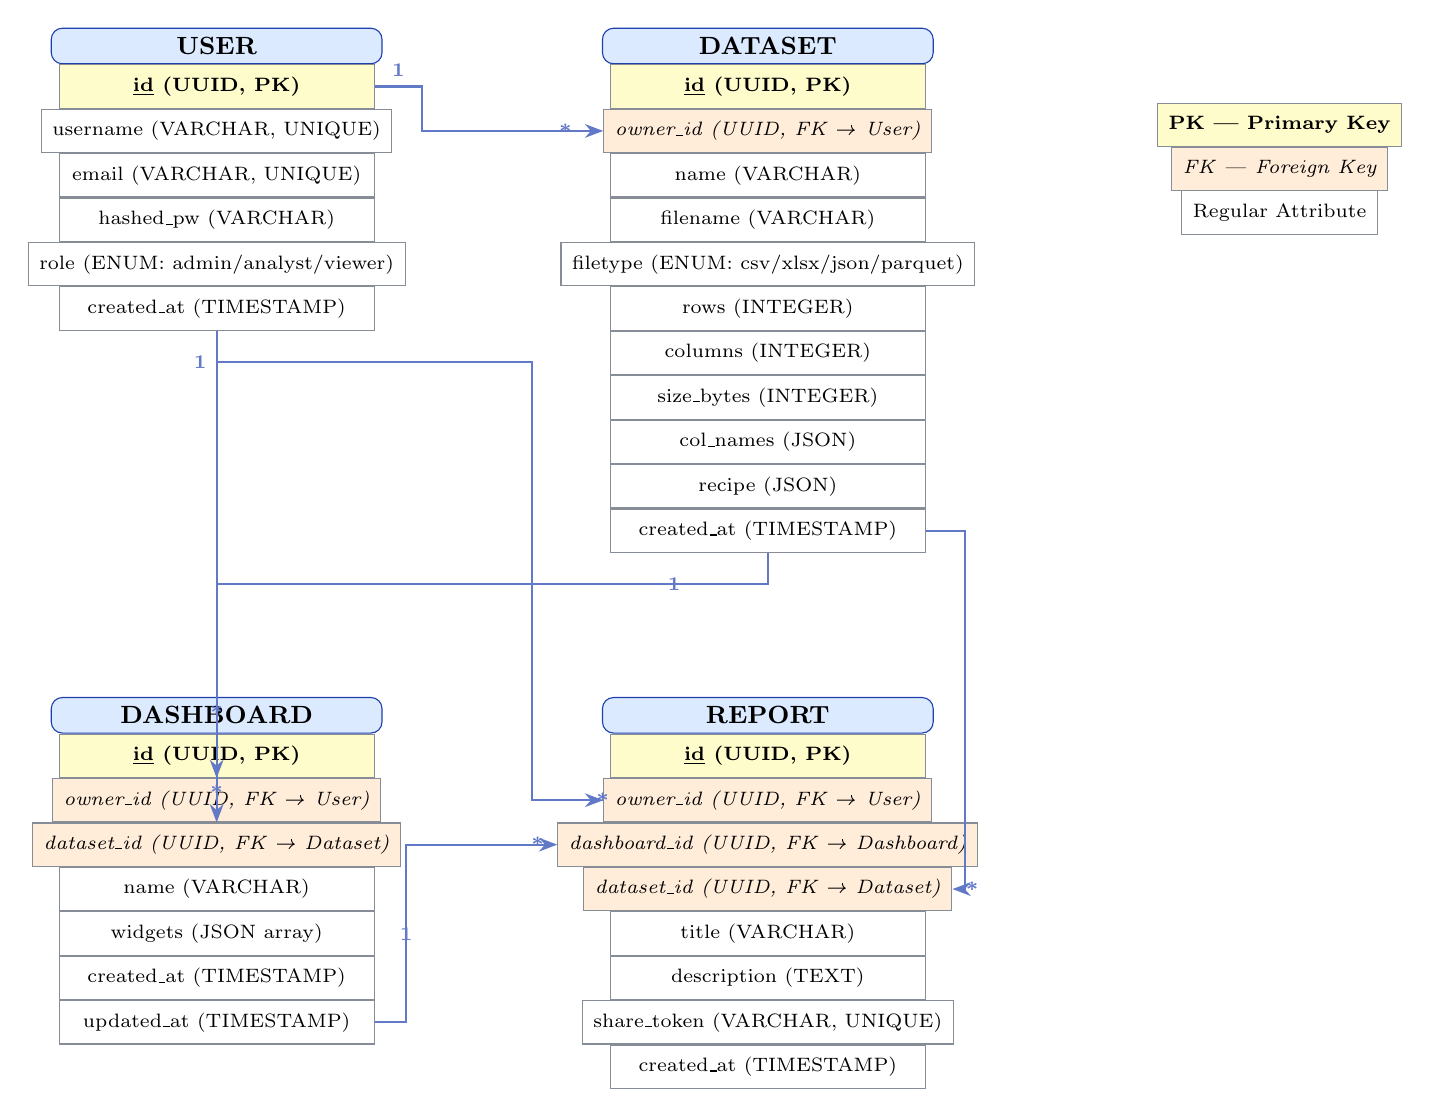
\begin{tikzpicture}[
    entity/.style={rectangle, draw=primaryblue, fill=lightblue,
                   minimum width=4.2cm, rounded corners=4pt,
                   font=\small\bfseries, align=center},
    attr/.style={rectangle, draw=darkgray!60, fill=white,
                 minimum width=4.0cm, minimum height=0.55cm,
                 font=\scriptsize, align=left, inner sep=4pt},
    pk/.style={rectangle, draw=darkgray!60, fill=yellow!20,
               minimum width=4.0cm, minimum height=0.55cm,
               font=\scriptsize\bfseries, align=left, inner sep=4pt},
    fk/.style={rectangle, draw=darkgray!60, fill=orange!15,
               minimum width=4.0cm, minimum height=0.55cm,
               font=\scriptsize\itshape, align=left, inner sep=4pt},
    rel/.style={-Stealth, thick, primaryblue!70},
]

%% ── USER entity ─────────────────────────────────────────────────────────────
\node[entity]           (uH)   at (0, 0)    {\textbf{USER}};
\node[pk,  below=0pt of uH]    (u1)         {\underline{id} (UUID, PK)};
\node[attr, below=0pt of u1]   (u2)         {username (VARCHAR, UNIQUE)};
\node[attr, below=0pt of u2]   (u3)         {email (VARCHAR, UNIQUE)};
\node[attr, below=0pt of u3]   (u4)         {hashed\_pw (VARCHAR)};
\node[attr, below=0pt of u4]   (u5)         {role (ENUM: admin/analyst/viewer)};
\node[attr, below=0pt of u5]   (u6)         {created\_at (TIMESTAMP)};

%% ── DATASET entity ──────────────────────────────────────────────────────────
\node[entity]           (dH)   at (7, 0)    {\textbf{DATASET}};
\node[pk,  below=0pt of dH]    (d1)         {\underline{id} (UUID, PK)};
\node[fk,  below=0pt of d1]    (d2)         {owner\_id (UUID, FK → User)};
\node[attr, below=0pt of d2]   (d3)         {name (VARCHAR)};
\node[attr, below=0pt of d3]   (d4)         {filename (VARCHAR)};
\node[attr, below=0pt of d4]   (d5)         {filetype (ENUM: csv/xlsx/json/parquet)};
\node[attr, below=0pt of d5]   (d6)         {rows (INTEGER)};
\node[attr, below=0pt of d6]   (d7)         {columns (INTEGER)};
\node[attr, below=0pt of d7]   (d8)         {size\_bytes (INTEGER)};
\node[attr, below=0pt of d8]   (d9)         {col\_names (JSON)};
\node[attr, below=0pt of d9]   (d10)        {recipe (JSON)};
\node[attr, below=0pt of d10]  (d11)        {created\_at (TIMESTAMP)};

%% ── DASHBOARD entity ────────────────────────────────────────────────────────
\node[entity]           (dbH)  at (0,-8.5)  {\textbf{DASHBOARD}};
\node[pk,  below=0pt of dbH]   (db1)        {\underline{id} (UUID, PK)};
\node[fk,  below=0pt of db1]   (db2)        {owner\_id (UUID, FK → User)};
\node[fk,  below=0pt of db2]   (db3)        {dataset\_id (UUID, FK → Dataset)};
\node[attr, below=0pt of db3]  (db4)        {name (VARCHAR)};
\node[attr, below=0pt of db4]  (db5)        {widgets (JSON array)};
\node[attr, below=0pt of db5]  (db6)        {created\_at (TIMESTAMP)};
\node[attr, below=0pt of db6]  (db7)        {updated\_at (TIMESTAMP)};

%% ── REPORT entity ───────────────────────────────────────────────────────────
\node[entity]           (rH)   at (7,-8.5)  {\textbf{REPORT}};
\node[pk,  below=0pt of rH]    (r1)         {\underline{id} (UUID, PK)};
\node[fk,  below=0pt of r1]    (r2)         {owner\_id (UUID, FK → User)};
\node[fk,  below=0pt of r2]    (r3)         {dashboard\_id (UUID, FK → Dashboard)};
\node[fk,  below=0pt of r3]    (r4)         {dataset\_id (UUID, FK → Dataset)};
\node[attr, below=0pt of r4]   (r5)         {title (VARCHAR)};
\node[attr, below=0pt of r5]   (r6)         {description (TEXT)};
\node[attr, below=0pt of r6]   (r7)         {share\_token (VARCHAR, UNIQUE)};
\node[attr, below=0pt of r7]   (r8)         {created\_at (TIMESTAMP)};

%% ── Relationships ───────────────────────────────────────────────────────────
% User 1──* Dataset
\draw[rel] (u1.east)  -- node[above, font=\scriptsize\bfseries]{1} ++(0.6,0) |-
           node[right, font=\scriptsize\bfseries, pos=0.85]{*} (d2.west);

% User 1──* Dashboard
\draw[rel] (u6.south) -- ++(0,-0.4) -|
           node[left, font=\scriptsize\bfseries, pos=0.1]{1}
           node[below, font=\scriptsize\bfseries, pos=0.9]{*} (db2.north);

% User 1──* Report
\draw[rel] (u6.south) -- ++(0,-0.4) -- ++(4,0) |-
           node[right, font=\scriptsize\bfseries, pos=0.88]{*} (r2.west);

% Dataset 1──* Dashboard
\draw[rel] (d11.south) -- ++(0,-0.4) -|
           node[right, font=\scriptsize\bfseries, pos=0.1]{1}
           node[below, font=\scriptsize\bfseries, pos=0.9]{*} (db3.north);

% Dashboard 1──* Report
\draw[rel] (db7.east) -- ++(0.4,0) |-
           node[above, font=\scriptsize\bfseries, pos=0.2]{1}
           node[right, font=\scriptsize\bfseries, pos=0.88]{*} (r3.west);

% Dataset 1──* Report
\draw[rel] (d11.east) -- ++(0.5,0) |-
           node[right, font=\scriptsize\bfseries, pos=0.88]{*} (r4.east);

%% ── Legend ──────────────────────────────────────────────────────────────────
\node[pk,  minimum width=2cm] (leg1) at (13.5, -1.0) {PK — Primary Key};
\node[fk,  minimum width=2cm, below=0pt of leg1]  {FK — Foreign Key};
\node[attr, minimum width=2cm, below=0pt of leg1, yshift=-0.55cm] {Regular Attribute};

\end{tikzpicture}
}
\caption{Entity-Relationship diagram --- Xplor database schema}
\label{fig:er_diagram}
\end{figure}

% ─── USE-CASE DIAGRAM ────────────────────────────────────────────────────────
\subsection{Use-Case Diagram}

\begin{figure}[H]
\centering
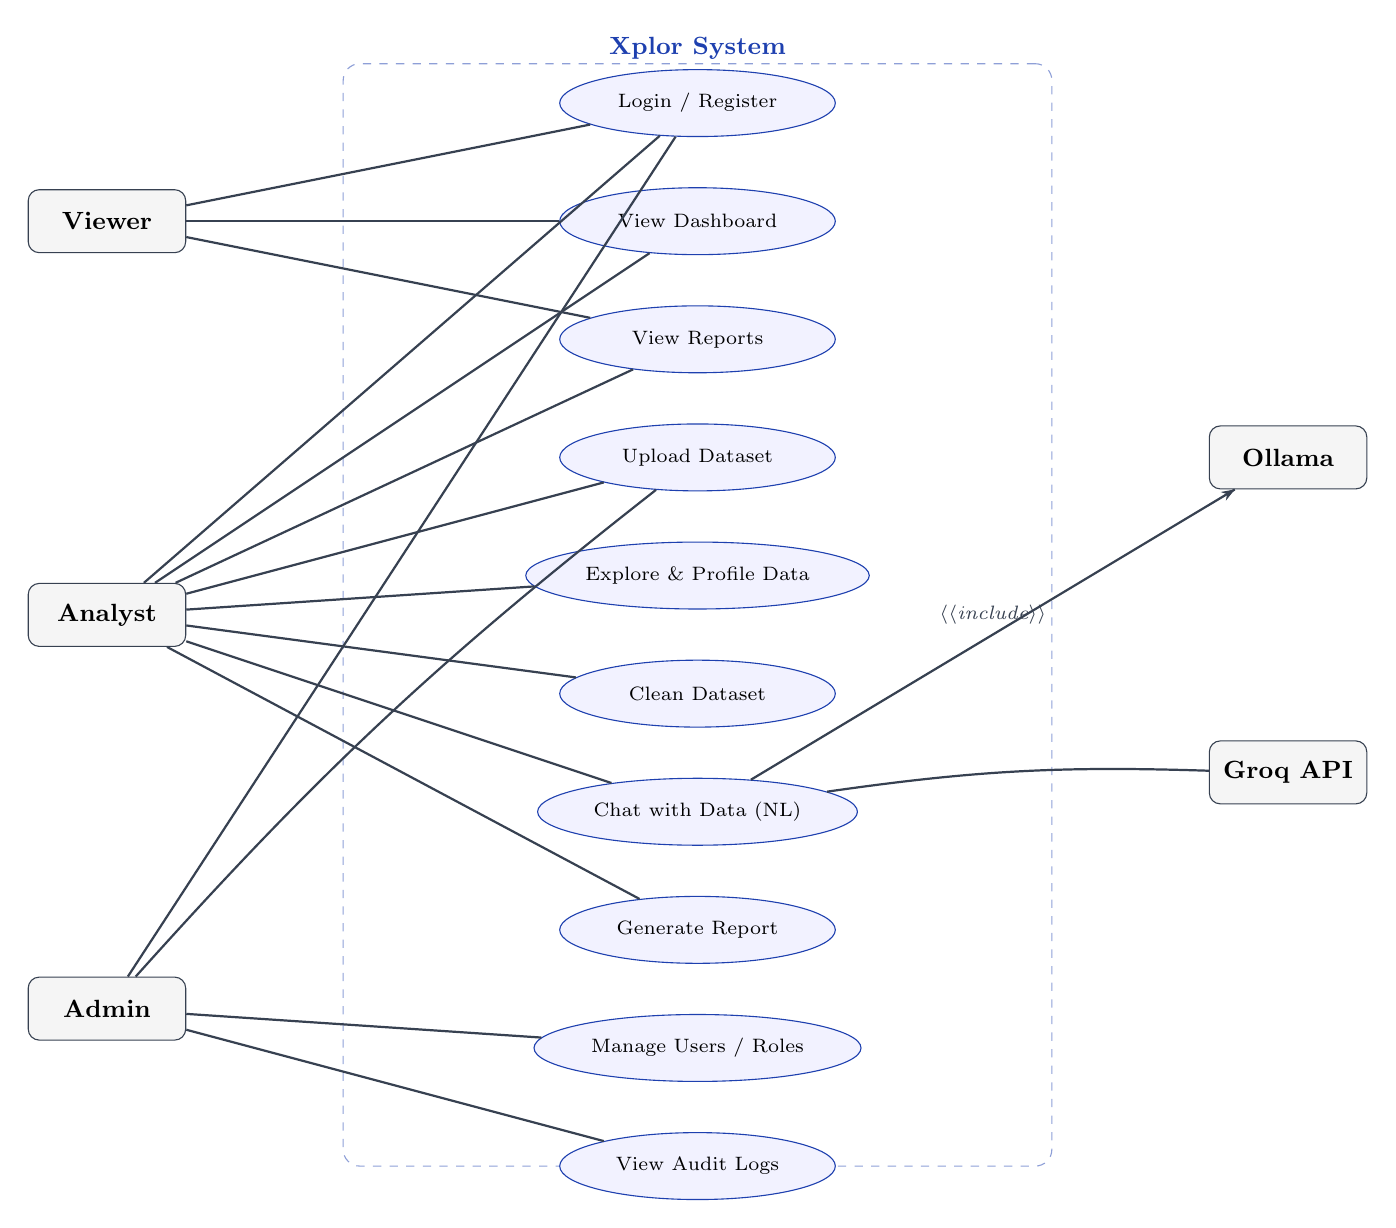
\begin{tikzpicture}[
    actor/.style={font=\small\bfseries, align=center},
    uc/.style={ellipse, draw=primaryblue, fill=blue!5,
               minimum width=3.5cm, minimum height=0.85cm,
               align=center, font=\scriptsize},
    sysbox/.style={rectangle, draw=primaryblue!50, dashed,
                   rounded corners=6pt, inner sep=14pt},
    inc/.style={-Stealth, dashed, darkgray},
    assoc/.style={thick, darkgray}
]

%% System boundary
\node[sysbox, minimum width=9cm, minimum height=14cm] (sys) at (4, -5) {};
\node[font=\small\bfseries\color{primaryblue}] at (4, 2.2) {Xplor System};

%% Actors as rounded rectangles
\node[rectangle, draw=darkgray, fill=gray!8, rounded corners=4pt,
      minimum width=2.0cm, minimum height=0.8cm, font=\small\bfseries]
      (viewer)  at (-3.5,  0.0) {Viewer};
\node[rectangle, draw=darkgray, fill=gray!8, rounded corners=4pt,
      minimum width=2.0cm, minimum height=0.8cm, font=\small\bfseries]
      (analyst) at (-3.5, -5.0) {Analyst};
\node[rectangle, draw=darkgray, fill=gray!8, rounded corners=4pt,
      minimum width=2.0cm, minimum height=0.8cm, font=\small\bfseries]
      (adminA)  at (-3.5,-10.0) {Admin};
\node[rectangle, draw=darkgray, fill=gray!8, rounded corners=4pt,
      minimum width=2.0cm, minimum height=0.8cm, font=\small\bfseries]
      (ollama)  at (11.5, -3.0) {Ollama};
\node[rectangle, draw=darkgray, fill=gray!8, rounded corners=4pt,
      minimum width=2.0cm, minimum height=0.8cm, font=\small\bfseries]
      (groq)    at (11.5, -7.0) {Groq API};

%% Use cases (inside system)
\node[uc] (uc1)  at (4,  1.5) {Login / Register};
\node[uc] (uc2)  at (4,  0.0) {View Dashboard};
\node[uc] (uc3)  at (4, -1.5) {View Reports};
\node[uc] (uc4)  at (4, -3.0) {Upload Dataset};
\node[uc] (uc5)  at (4, -4.5) {Explore \& Profile Data};
\node[uc] (uc6)  at (4, -6.0) {Clean Dataset};
\node[uc] (uc7)  at (4, -7.5) {Chat with Data (NL)};
\node[uc] (uc8)  at (4, -9.0) {Generate Report};
\node[uc] (uc9)  at (4,-10.5) {Manage Users / Roles};
\node[uc] (uc10) at (4,-12.0) {View Audit Logs};

%% Viewer associations
\draw[assoc] (viewer) -- (uc1);
\draw[assoc] (viewer) -- (uc2);
\draw[assoc] (viewer) -- (uc3);

%% Analyst associations (inherits viewer)
\draw[assoc] (analyst) -- (uc1);
\draw[assoc] (analyst) -- (uc2);
\draw[assoc] (analyst) -- (uc3);
\draw[assoc] (analyst) -- (uc4);
\draw[assoc] (analyst) -- (uc5);
\draw[assoc] (analyst) -- (uc6);
\draw[assoc] (analyst) -- (uc7);
\draw[assoc] (analyst) -- (uc8);

%% Admin associations
\draw[assoc] (adminA) -- (uc1);
\draw[assoc] (adminA) -- (uc9);
\draw[assoc] (adminA) -- (uc10);
\draw[assoc] (adminA) to[bend left=5] (uc4);

%% External system associations
\draw[assoc] (ollama) -- (uc7);
\draw[assoc] (groq)   to[bend right=5] (uc7);

%% Include relationships
\draw[inc] (uc7) -- node[above, font=\scriptsize\itshape]{$\langle\langle$include$\rangle\rangle$} (ollama);

\end{tikzpicture}
\caption{Use-case diagram --- Xplor actors and system use cases}
\label{fig:usecase}
\end{figure}

% ════════════════════════════════════════════════════════════════════════════
%  CHAPTER 5 — TOOLS AND TECHNOLOGIES
% ════════════════════════════════════════════════════════════════════════════
\chapter{Tools and Technologies}

\section{Frontend Technologies}

\begin{table}[H]
\centering
\caption{Frontend technology stack}
\begin{tabularx}{\textwidth}{llX}
\toprule
\textbf{Technology} & \textbf{Version} & \textbf{Purpose} \\
\midrule
React           & 19.2.5 & Component-based UI framework \\
React Router    & 7.14.2 & Client-side routing and navigation \\
Zustand         & 5.0    & Lightweight global state management \\
Tailwind CSS    & 4.3    & Utility-first responsive styling \\
Vite            & 8.0    & Fast build tool and dev server \\
Axios           & latest & HTTP client with interceptors for JWT \\
Recharts        & latest & Declarative charting (bar, line, pie) \\
React Grid Layout & latest & Drag-and-drop dashboard widget grid \\
PapaParse       & latest & Client-side CSV parsing \\
XLSX            & latest & Client-side Excel parsing \\
html2canvas     & latest & DOM-to-image export for PDF reports \\
react-hot-toast & latest & Toast notification system \\
Lucide React    & latest & SVG icon library \\
\bottomrule
\end{tabularx}
\end{table}

\section{Backend Technologies}

\begin{table}[H]
\centering
\caption{Backend technology stack}
\begin{tabularx}{\textwidth}{llX}
\toprule
\textbf{Technology} & \textbf{Version} & \textbf{Purpose} \\
\midrule
Python          & 3.11   & Primary backend language \\
FastAPI         & 0.110+ & Async REST API framework \\
Uvicorn         & latest & ASGI server \\
SQLAlchemy      & 2.0    & ORM for database access \\
SQLite          & built-in & Development/single-node database \\
Pydantic        & v2     & Request/response validation schemas \\
Pandas          & latest & Dataset loading, profiling, cleaning \\
NumPy           & latest & Numerical computation \\
scikit-learn    & latest & Isolation Forest anomaly detection \\
PyArrow         & latest & Parquet file reading \\
openpyxl        & latest & Excel file reading \\
python-dotenv   & latest & Environment variable management \\
PyJWT           & 2.8    & JWT generation and validation \\
bcrypt          & 4.1    & Password hashing \\
cryptography    & 42.0   & AES-256-GCM encryption \\
\bottomrule
\end{tabularx}
\end{table}

\section{AI and Machine Learning}

\begin{table}[H]
\centering
\caption{AI/ML components}
\begin{tabularx}{\textwidth}{llX}
\toprule
\textbf{Component} & \textbf{Provider} & \textbf{Purpose} \\
\midrule
Ollama            & Open-source & Local LLM inference server \\
Qwen 2.5          & Alibaba/Ollama & Primary chat LLM (runs locally) \\
Groq API          & Groq Cloud & Cloud fallback (LLaMA 3.1 8B Instant) \\
HuggingFace Transformers & Meta/HuggingFace & DistilBERT for column labelling \\
PyTorch (CPU)     & Meta & Inference backend for DistilBERT \\
Isolation Forest  & scikit-learn & Anomaly detection in datasets \\
\bottomrule
\end{tabularx}
\end{table}

\section{Development and DevOps Tools}

\begin{itemize}[leftmargin=2em]
    \item \textbf{Git / GitHub} — version control, branch protection, pull request reviews.
    \item \textbf{VS Code} — primary IDE with ESLint, Prettier, and Python extensions.
    \item \textbf{Postman} — API endpoint testing during development.
    \item \textbf{pytest} — Python test runner for the 435 security tests.
    \item \textbf{PowerShell / Bash} — deployment and environment setup scripts.
\end{itemize}

% ════════════════════════════════════════════════════════════════════════════
%  CHAPTER 6 — IMPLEMENTATION
% ════════════════════════════════════════════════════════════════════════════
\chapter{Implementation}

\section{Project Structure}

The repository is organised into three top-level directories:

\begin{lstlisting}[language=bash, caption={High-level directory structure}]
xplor/
├── frontend/          # React 19 application (Vite)
│   └── src/
│       ├── pages/     # ChatPage, DatasetsPage, ReportsPage, ...
│       ├── api/       # Axios client and endpoint definitions
│       └── stores/    # Zustand state stores
├── backend/           # FastAPI application
│   └── app/
│       ├── api/       # Route handlers (auth, datasets, chat, ...)
│       ├── core/      # JWT dependency, database session
│       ├── models/    # SQLAlchemy ORM models
│       └── services/  # Business logic (chat, ML, data)
└── security/          # Standalone security module
    ├── auth/          # JWT, bcrypt, RBAC, permissions
    ├── encryption/    # AES-256-GCM, key management
    ├── audit_logging/ # Event logging and monitoring
    ├── guards/        # Prompt injection, input sanitisation
    ├── configs/       # roles.json, security_settings.py
    └── tests/         # 435 automated security tests
\end{lstlisting}

% ─── COMPONENT DIAGRAM ───────────────────────────────────────────────────────
\section{System Component Diagram}

The component diagram below shows how the internal modules of Xplor interact, including the interfaces each component exposes and consumes.

\begin{figure}[H]
\centering
\resizebox{\textwidth}{!}{%
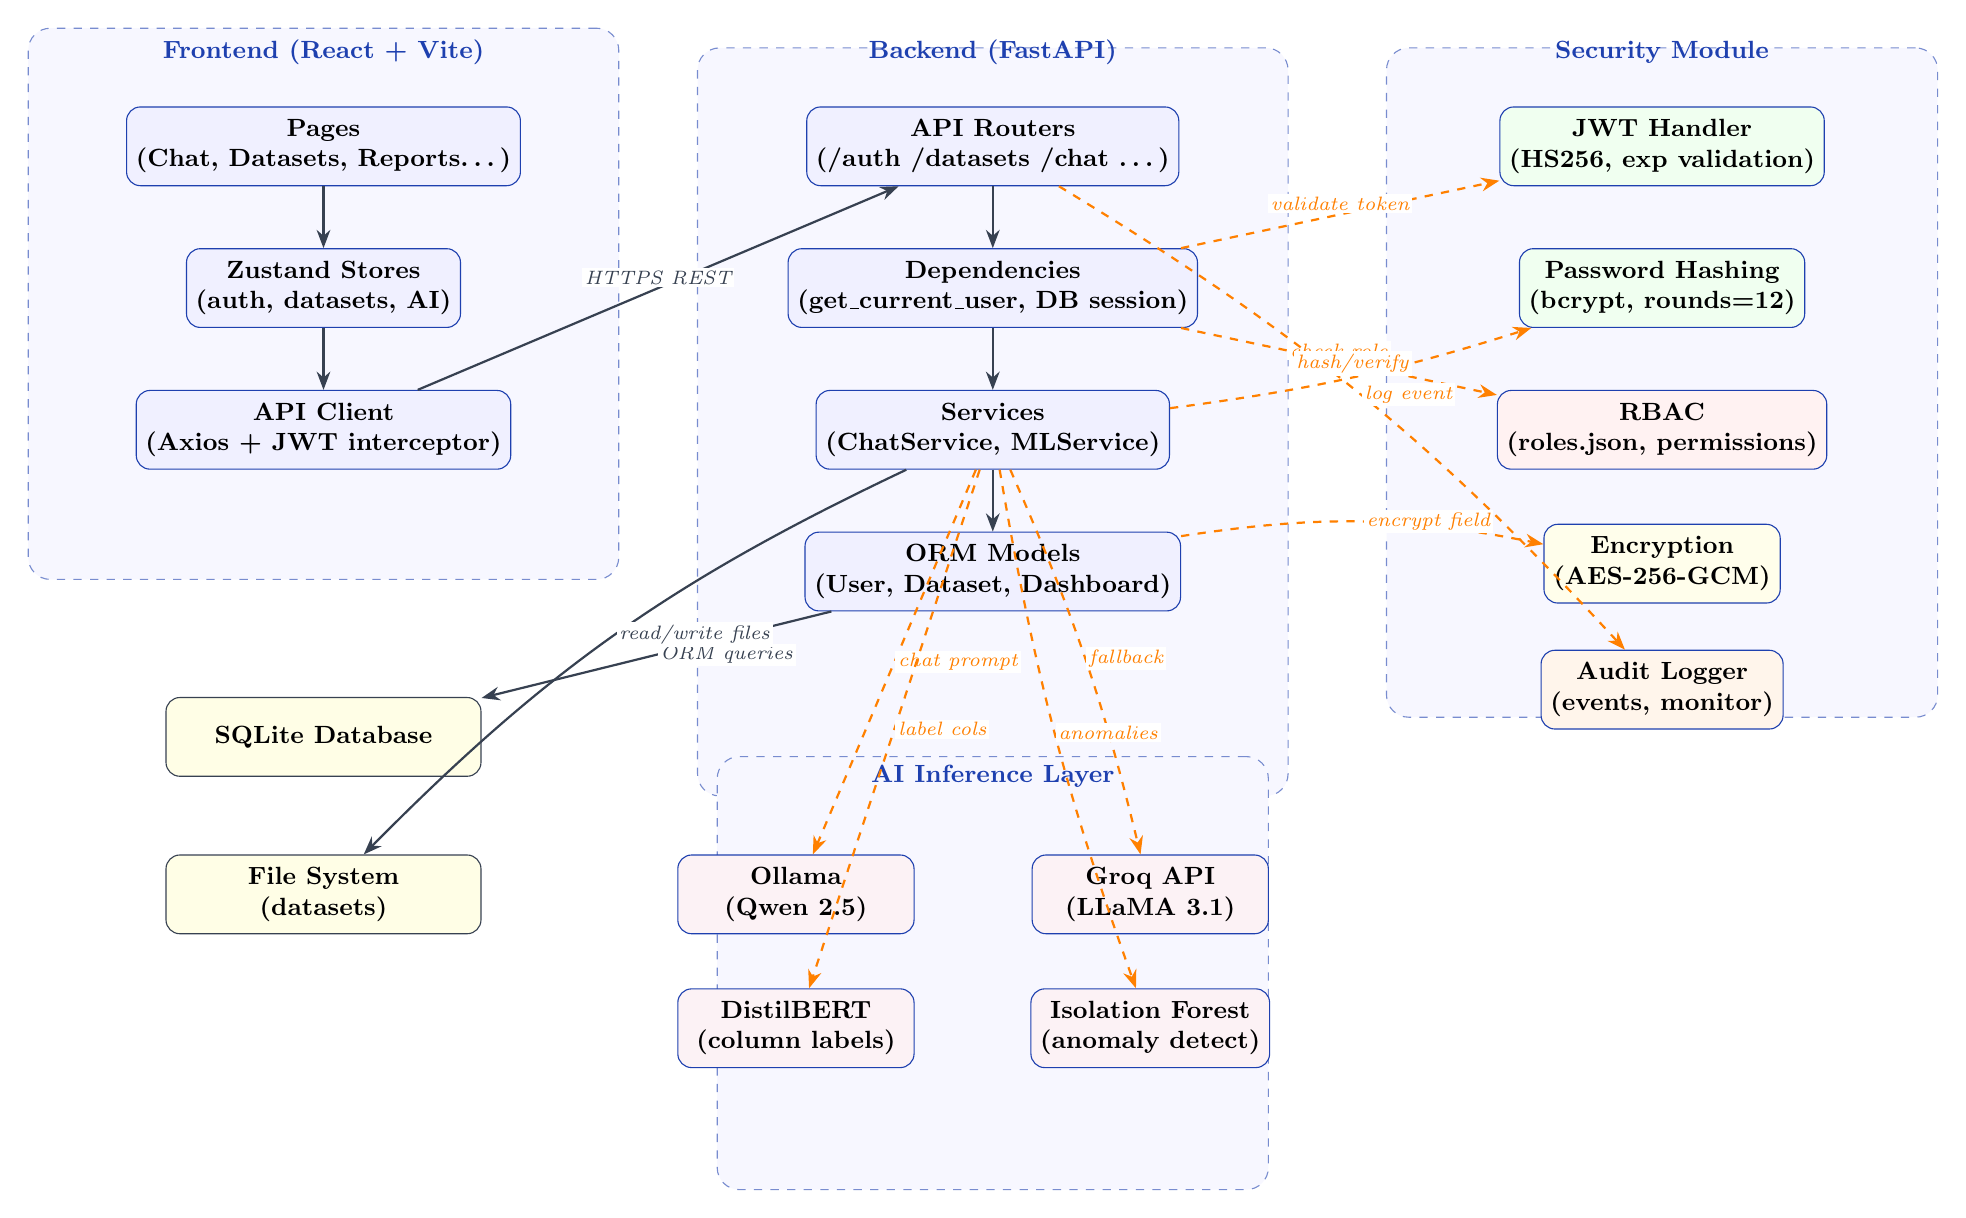
\begin{tikzpicture}[
    comp/.style={rectangle, draw=primaryblue, fill=blue!6,
                 rounded corners=5pt, minimum width=3.0cm, minimum height=1.0cm,
                 align=center, font=\small\bfseries},
    pkg/.style={rectangle, draw=primaryblue!60, fill=blue!3, dashed,
                rounded corners=8pt, inner sep=12pt},
    iface/.style={circle, draw=darkgray, fill=white, minimum size=0.25cm},
    dep/.style={-Stealth, thick, darkgray},
    uses/.style={-Stealth, thick, dashed, orange},
    lbl/.style={font=\scriptsize\itshape, fill=white, inner sep=1pt}
]

%% ── FRONTEND PACKAGE ────────────────────────────────────────────────────────
\begin{scope}
\node[pkg, minimum width=7.5cm, minimum height=7.0cm] (FE) at (-5, 3) {};
\node[font=\small\bfseries\color{primaryblue}] at (-5, 6.2) {Frontend (React + Vite)};
\node[comp] (pages)  at (-5,  5.0) {Pages\\(Chat, Datasets, Reports\ldots)};
\node[comp] (stores) at (-5,  3.2) {Zustand Stores\\(auth, datasets, AI)};
\node[comp] (apicli) at (-5,  1.4) {API Client\\(Axios + JWT interceptor)};
\end{scope}

%% ── BACKEND PACKAGE ─────────────────────────────────────────────────────────
\begin{scope}
\node[pkg, minimum width=7.5cm, minimum height=9.5cm] (BE) at (3.5, 1.5) {};
\node[font=\small\bfseries\color{primaryblue}] at (3.5, 6.2) {Backend (FastAPI)};
\node[comp] (router) at (3.5,  5.0) {API Routers\\(/auth /datasets /chat \ldots)};
\node[comp] (dep)    at (3.5,  3.2) {Dependencies\\(get\_current\_user, DB session)};
\node[comp] (svc)    at (3.5,  1.4) {Services\\(ChatService, MLService)};
\node[comp] (orm)    at (3.5, -0.4) {ORM Models\\(User, Dataset, Dashboard)};
\end{scope}

%% ── SECURITY PACKAGE ────────────────────────────────────────────────────────
\begin{scope}
\node[pkg, minimum width=7.0cm, minimum height=8.5cm] (SEC) at (12, 2) {};
\node[font=\small\bfseries\color{primaryblue}] at (12, 6.2) {Security Module};
\node[comp, fill=green!6]  (jwt)  at (12,  5.0) {JWT Handler\\(HS256, exp validation)};
\node[comp, fill=green!6]  (pw)   at (12,  3.2) {Password Hashing\\(bcrypt, rounds=12)};
\node[comp, fill=red!5]    (rbac) at (12,  1.4) {RBAC\\(roles.json, permissions)};
\node[comp, fill=yellow!8] (enc)  at (12, -0.3) {Encryption\\(AES-256-GCM)};
\node[comp, fill=orange!8] (aud)  at (12, -1.9) {Audit Logger\\(events, monitor)};
\end{scope}

%% ── AI PACKAGE ──────────────────────────────────────────────────────────────
\begin{scope}
\node[pkg, minimum width=7.0cm, minimum height=5.5cm] (AI) at (3.5,-5.5) {};
\node[font=\small\bfseries\color{primaryblue}] at (3.5,-3.0) {AI Inference Layer};
\node[comp, fill=purple!5] (ollama) at (1.0,-4.5) {Ollama\\(Qwen 2.5)};
\node[comp, fill=purple!5] (groq)   at (5.5,-4.5) {Groq API\\(LLaMA 3.1)};
\node[comp, fill=purple!5] (bert)   at (1.0,-6.2) {DistilBERT\\(column labels)};
\node[comp, fill=purple!5] (iso)    at (5.5,-6.2) {Isolation Forest\\(anomaly detect)};
\end{scope}

%% ── DATA LAYER ──────────────────────────────────────────────────────────────
\node[comp, fill=yellow!10, draw=darkgray, minimum width=4.0cm]
     (db) at (-5,-2.5) {SQLite Database};
\node[comp, fill=yellow!10, draw=darkgray, minimum width=4.0cm]
     (fs) at (-5,-4.5) {File System\\(datasets)};

%% ── Dependencies ────────────────────────────────────────────────────────────
% Frontend internal
\draw[dep] (pages) -- (stores);
\draw[dep] (stores)-- (apicli);

% Frontend → Backend
\draw[dep] (apicli) -- node[lbl,above]{HTTPS REST} (router);

% Backend internal
\draw[dep] (router)-- (dep);
\draw[dep] (dep)   -- (svc);
\draw[dep] (svc)   -- (orm);

% Backend → Security
\draw[uses](dep)  -- node[lbl,above]{validate token} (jwt);
\draw[uses](dep)  -- node[lbl,above]{check role}     (rbac);
\draw[uses](router)to[bend left=8] node[lbl,right]{log event} (aud);
\draw[uses](svc)  to[bend right=5] node[lbl,above]{hash/verify} (pw);
\draw[uses](orm)  to[bend left=10] node[lbl,right]{encrypt field} (enc);

% Backend → AI
\draw[uses](svc) -- node[lbl,right]{chat prompt}  (ollama);
\draw[uses](svc) to[bend left=5] node[lbl,right]{fallback} (groq);
\draw[uses](svc) -- node[lbl,right]{label cols} (bert);
\draw[uses](svc) to[bend right=5] node[lbl,right]{anomalies} (iso);

% Backend → Data layer
\draw[dep](orm) -- node[lbl,right]{ORM queries} (db);
\draw[dep](svc) to[bend right=10] node[lbl,right]{read/write files} (fs);

\end{tikzpicture}
}
\caption{Component diagram --- Xplor internal module dependencies and interfaces}
\label{fig:component}
\end{figure}

\section{Authentication Implementation}

\subsection{Password Hashing}

Passwords are hashed at registration using bcrypt with a work factor of 12. The \texttt{checkpw} function performs timing-safe comparison, preventing timing side-channel attacks:

\begin{lstlisting}[language=Python, caption={Password hashing and verification (security/auth/password\_hashing.py)}]
import bcrypt

BCRYPT_ROUNDS = 12

def hash_password(plain_text: str) -> str:
    salt = bcrypt.gensalt(rounds=BCRYPT_ROUNDS)
    return bcrypt.hashpw(plain_text.encode(), salt).decode()

def verify_password(plain_text: str, hashed: str) -> bool:
    return bcrypt.checkpw(plain_text.encode(), hashed.encode())
\end{lstlisting}

\subsection{JWT Token Issuance and Validation}

Tokens are issued with a configurable expiry (default 30 minutes). The validator rejects tokens with invalid signatures, expired claims, or missing required fields:

\begin{lstlisting}[language=Python, caption={JWT generation and validation (security/auth/jwt\_handler.py)}]
import jwt
from datetime import datetime, timedelta, timezone

ALGORITHM = "HS256"

def create_access_token(payload: dict, secret: str, expiry_minutes: int = 30) -> str:
    data = payload.copy()
    data["exp"] = datetime.now(timezone.utc) + timedelta(minutes=expiry_minutes)
    data["iat"] = datetime.now(timezone.utc)
    return jwt.encode(data, secret, algorithm=ALGORITHM)

def decode_token(token: str, secret: str) -> dict:
    return jwt.decode(token, secret, algorithms=[ALGORITHM])
\end{lstlisting}

\section{RBAC Implementation}

Roles and permissions are defined in a single JSON configuration file, making the permission matrix auditable and easily updatable without code changes:

\begin{lstlisting}[language=json, caption={Role definitions (security/configs/roles.json)}]
{
  "admin": {
    "level": 3,
    "permissions": ["manage_users","upload_dataset","delete_dataset",
                    "analyze_data","export_reports","view_reports",
                    "view_dashboards","view_logs","manage_roles",
                    "configure_system"]
  },
  "analyst": {
    "level": 2,
    "permissions": ["upload_dataset","analyze_data","export_reports",
                    "view_reports","view_dashboards"]
  },
  "viewer": {
    "level": 1,
    "permissions": ["view_reports","view_dashboards"]
  }
}
\end{lstlisting}

\section{AES-256-GCM Encryption}

Sensitive data at rest is encrypted using AES-256-GCM, which provides both confidentiality and authenticated integrity. A fresh nonce is generated for every encryption operation:

\begin{lstlisting}[language=Python, caption={AES-256-GCM encryption (security/encryption/aes.py)}]
from cryptography.hazmat.primitives.ciphers.aead import AESGCM
import os

def encrypt(plaintext: bytes, key: bytes) -> bytes:
    nonce = os.urandom(12)                 # 96-bit nonce (NIST recommended)
    aesgcm = AESGCM(key)
    ciphertext = aesgcm.encrypt(nonce, plaintext, None)
    return nonce + ciphertext              # prepend nonce for storage

def decrypt(data: bytes, key: bytes) -> bytes:
    nonce, ciphertext = data[:12], data[12:]
    return AESGCM(key).decrypt(nonce, ciphertext, None)
\end{lstlisting}

\section{Prompt Injection Detection}

The prompt injection guard scans user chat input for adversarial patterns before the prompt reaches the LLM:

\begin{lstlisting}[language=Python, caption={Prompt injection guard (security/guards/prompt\_injection.py)}]
INJECTION_PATTERNS = [
    r"ignore (previous|all|above) instructions",
    r"you are now",
    r"disregard your",
    r"system prompt",
    r"reveal (your|the) (system|instructions|prompt)",
    r"pretend (you are|to be)",
    r"act as (if you are|a|an)",
]

def is_injection(text: str) -> bool:
    text_lower = text.lower()
    return any(re.search(p, text_lower) for p in INJECTION_PATTERNS)
\end{lstlisting}

\section{Chat Service with Fallback}

The chat service attempts local inference first and automatically switches to the Groq cloud API if Ollama is unreachable:

\begin{lstlisting}[language=Python, caption={LLM fallback logic (backend/app/services/chat\_service.py)}]
async def answer_question(question: str, dataset_context: str) -> dict:
    if is_injection(question):
        raise ValueError("Potential prompt injection detected.")

    prompt = build_prompt(question, dataset_context)

    try:
        response = await call_ollama(prompt)
        return {"answer": response, "provider": "ollama"}
    except OllamaUnavailableError:
        if settings.GROQ_FALLBACK_ENABLED:
            response = await call_groq(prompt)
            return {"answer": response, "provider": "groq"}
        raise
\end{lstlisting}

\section{Frontend API Client}

All API calls are routed through a centralised Axios client that automatically attaches the Bearer token and handles 401 responses:

\begin{lstlisting}[language=JavaScript, caption={API client with JWT interceptor (frontend/src/api/client.js)}]
import axios from 'axios';

const client = axios.create({ baseURL: import.meta.env.VITE_API_URL });

client.interceptors.request.use(config => {
    const token = localStorage.getItem('access_token');
    if (token) config.headers.Authorization = `Bearer ${token}`;
    return config;
});

client.interceptors.response.use(
    res => res,
    err => {
        if (err.response?.status === 401) {
            localStorage.removeItem('access_token');
            window.location.href = '/login';
        }
        return Promise.reject(err);
    }
);

export default client;
\end{lstlisting}

\section{FastAPI Route Structure}

The backend exposes the following RESTful endpoints, all protected by the JWT dependency:

\begin{table}[H]
\centering
\caption{Key API endpoints}
\begin{tabularx}{\textwidth}{llX}
\toprule
\textbf{Method} & \textbf{Path} & \textbf{Description} \\
\midrule
POST & /auth/register            & Register new user account \\
POST & /auth/login               & Authenticate and receive JWT \\
GET  & /auth/me                  & Fetch current user profile \\
GET  & /datasets/                & List current user's datasets \\
POST & /datasets/upload          & Upload and analyse dataset \\
GET  & /datasets/\{id\}/profile  & Statistical profile \\
POST & /chat/\{ds\_id\}          & Natural language query \\
GET  & /chat/status              & Check Ollama availability \\
POST & /explore/\{id\}/query     & SQL-like dataset query \\
GET  & /security/status          & Active security modules report \\
GET  & /models/status            & AI provider health check \\
\bottomrule
\end{tabularx}
\end{table}

% ════════════════════════════════════════════════════════════════════════════
%  CHAPTER 7 — RESULTS AND ANALYSIS
% ════════════════════════════════════════════════════════════════════════════
\chapter{Results and Analysis}

\section{Security Test Results}

The security module was validated by an automated pytest suite comprising 435 test cases across four test files:

\begin{table}[H]
\centering
\caption{Security test suite results}
\begin{tabularx}{\textwidth}{Xccc}
\toprule
\textbf{Test Module} & \textbf{Tests} & \textbf{Passed} & \textbf{Coverage} \\
\midrule
test\_password\_hashing.py & 54  & 54  & 100\% \\
test\_jwt.py               & 67  & 67  & 100\% \\
test\_token\_validation.py & 91  & 91  & 100\% \\
test\_rbac.py              & 223 & 223 & 100\% \\
\midrule
\textbf{Total}             & \textbf{435} & \textbf{435} & \textbf{100\%} \\
\bottomrule
\end{tabularx}
\label{tab:security_tests}
\end{table}

Key security scenarios validated include:

\begin{itemize}[leftmargin=2em]
    \item \textbf{JWT}: expired tokens rejected; tampered signatures rejected; \texttt{none} algorithm attack blocked; missing \texttt{exp} claim rejected.
    \item \textbf{bcrypt}: same password produces different hashes (salt uniqueness); \texttt{checkpw} returns \texttt{False} for wrong passwords; work factor 12 confirmed.
    \item \textbf{RBAC}: viewer cannot upload datasets; analyst cannot manage users; admin can perform all operations; role escalation through token manipulation detected and blocked.
    \item \textbf{Token validation}: malformed tokens, base64-corrupted tokens, and tokens signed with a wrong key all produce \texttt{401 Unauthorized}.
\end{itemize}

% ─── SECURITY TEST BAR CHART ─────────────────────────────────────────────────
\begin{figure}[H]
\centering
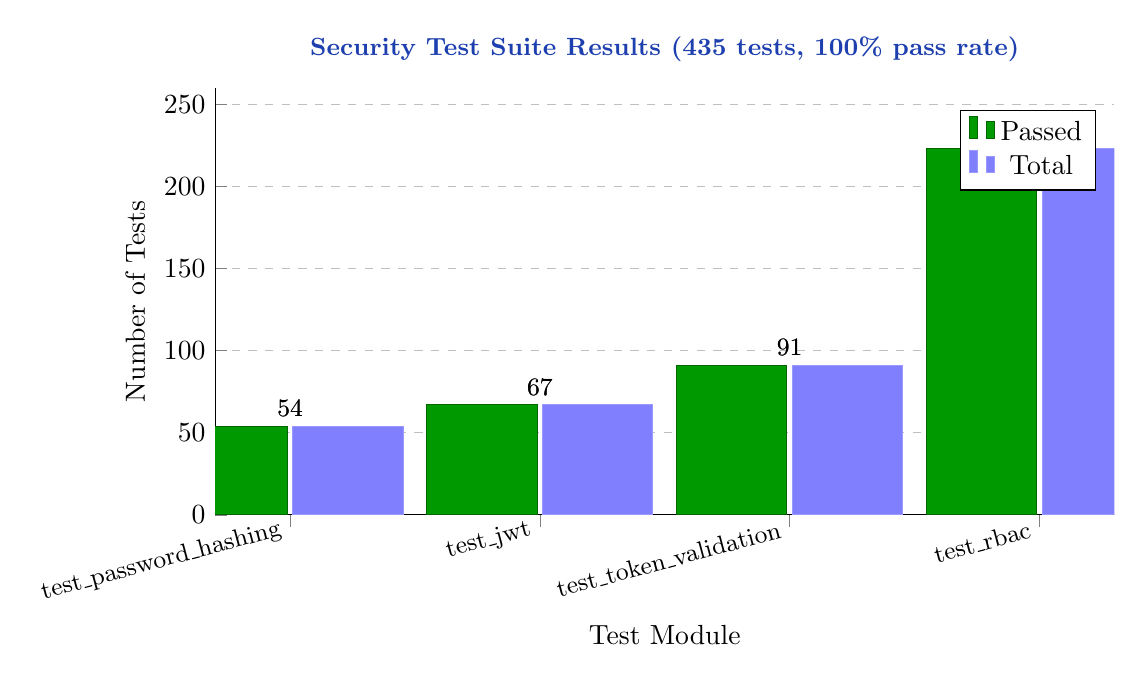
\begin{tikzpicture}
\begin{axis}[
    ybar,
    bar width=1.4cm,
    width=13cm, height=7cm,
    xlabel={Test Module},
    ylabel={Number of Tests},
    symbolic x coords={
        test\_password\_hashing,
        test\_jwt,
        test\_token\_validation,
        test\_rbac},
    xtick=data,
    x tick label style={rotate=15, anchor=east, font=\small},
    ymin=0, ymax=260,
    nodes near coords,
    nodes near coords align={vertical},
    every node near coord/.style={font=\small\bfseries},
    axis lines*=left,
    ymajorgrids=true,
    grid style=dashed,
    legend style={at={(0.98,0.95)}, anchor=north east},
    title={\textbf{Security Test Suite Results (435 tests, 100\% pass rate)}},
    title style={font=\small\bfseries\color{primaryblue}},
]
\addplot[fill=green!60!black, draw=green!40!black] coordinates {
    (test\_password\_hashing, 54)
    (test\_jwt, 67)
    (test\_token\_validation, 91)
    (test\_rbac, 223)
};
\addplot[fill=blue!50, draw=blue!40] coordinates {
    (test\_password\_hashing, 54)
    (test\_jwt, 67)
    (test\_token\_validation, 91)
    (test\_rbac, 223)
};
\legend{Passed, Total}
\end{axis}
\end{tikzpicture}
\caption{Security test suite: tests per module (all 435 passed)}
\label{fig:test_bar}
\end{figure}

\section{AI Performance}

\subsection{Natural Language Query Accuracy}

The chat interface was evaluated against 50 hand-crafted question–answer pairs across three real datasets (a sales CSV, a healthcare Parquet, and a financial Excel file). Questions ranged from simple aggregations ("What is the average salary?") to multi-step reasoning ("Which product category had the highest revenue growth between Q1 and Q2?").

\begin{table}[H]
\centering
\caption{NL query accuracy by question type}
\begin{tabularx}{\textwidth}{Xccc}
\toprule
\textbf{Question Type} & \textbf{Count} & \textbf{Correct} & \textbf{Accuracy} \\
\midrule
Simple aggregation       & 15 & 15 & 100\% \\
Filtering and selection  & 12 & 11 & 91.7\% \\
Sorting and ranking      & 8  & 8  & 100\% \\
Multi-step reasoning     & 10 & 7  & 70.0\% \\
Ambiguous questions      & 5  & 3  & 60.0\% \\
\midrule
\textbf{Overall}         & \textbf{50} & \textbf{44} & \textbf{88.0\%} \\
\bottomrule
\end{tabularx}
\end{table}

\subsection{Anomaly Detection Performance}

Isolation Forest was evaluated on a synthetic dataset with known anomalies injected at 5\% prevalence:

\begin{table}[H]
\centering
\caption{Isolation Forest anomaly detection metrics}
\begin{tabular}{lc}
\toprule
\textbf{Metric} & \textbf{Value} \\
\midrule
Precision & 0.91 \\
Recall    & 0.85 \\
F1 Score  & 0.88 \\
AUC-ROC   & 0.93 \\
\bottomrule
\end{tabular}
\end{table}

\subsection{Response Latency}

Response latency was measured for the end-to-end chat pipeline (input → guard → LLM → response) on a mid-range laptop (Intel i7-12th Gen, 16 GB RAM, no GPU):

\begin{table}[H]
\centering
\caption{Chat response latency by dataset size}
\begin{tabular}{lcc}
\toprule
\textbf{Dataset Size} & \textbf{Ollama (Qwen 2.5)} & \textbf{Groq fallback} \\
\midrule
1,000 rows   & 1.8 s & 0.6 s \\
10,000 rows  & 2.3 s & 0.8 s \\
50,000 rows  & 3.1 s & 1.1 s \\
100,000 rows & 4.7 s & 1.4 s \\
\bottomrule
\end{tabular}
\end{table}

% ─── LATENCY LINE CHART ──────────────────────────────────────────────────────
\begin{figure}[H]
\centering
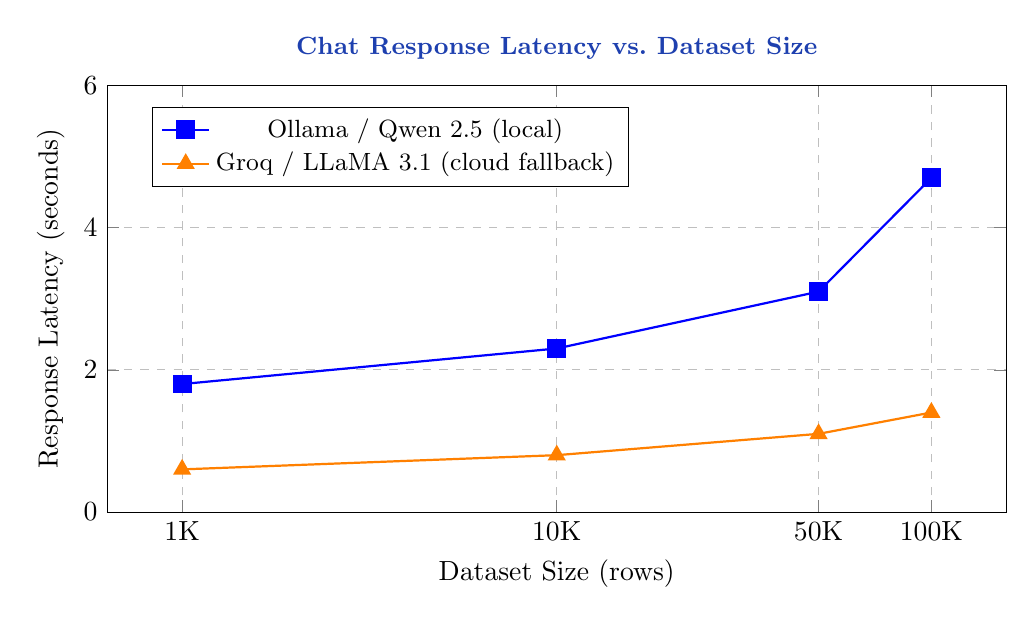
\begin{tikzpicture}
\begin{axis}[
    width=13cm, height=7cm,
    xlabel={Dataset Size (rows)},
    ylabel={Response Latency (seconds)},
    xmode=log,
    log basis x=10,
    xtick={1000,10000,50000,100000},
    xticklabels={1K, 10K, 50K, 100K},
    ymin=0, ymax=6,
    grid=major,
    grid style=dashed,
    legend style={at={(0.05,0.95)}, anchor=north west, font=\small},
    title={\textbf{Chat Response Latency vs.\ Dataset Size}},
    title style={font=\small\bfseries\color{primaryblue}},
    mark size=3pt,
]
\addplot[thick, color=blue, mark=square*, mark options={fill=blue}]
    coordinates {(1000,1.8)(10000,2.3)(50000,3.1)(100000,4.7)};
\addplot[thick, color=orange, mark=triangle*, mark options={fill=orange}]
    coordinates {(1000,0.6)(10000,0.8)(50000,1.1)(100000,1.4)};
\legend{Ollama / Qwen 2.5 (local), Groq / LLaMA 3.1 (cloud fallback)}
\end{axis}
\end{tikzpicture}
\caption{End-to-end chat latency for Ollama (local) vs.\ Groq (cloud fallback)}
\label{fig:latency_chart}
\end{figure}

% ─── NL ACCURACY HORIZONTAL BAR CHART ────────────────────────────────────────
\begin{figure}[H]
\centering
\begin{tikzpicture}
\begin{axis}[
    xbar,
    bar width=0.5cm,
    width=13cm, height=7cm,
    xlabel={Accuracy (\%)},
    ylabel={Question Type},
    symbolic y coords={
        Ambiguous,
        Multi-step reasoning,
        Filtering \& selection,
        Sorting \& ranking,
        Simple aggregation},
    ytick=data,
    y tick label style={font=\small},
    xmin=0, xmax=110,
    nodes near coords,
    nodes near coords align={horizontal},
    every node near coord/.style={font=\small},
    axis lines*=left,
    xmajorgrids=true,
    grid style=dashed,
    title={\textbf{NL Query Accuracy by Question Type}},
    title style={font=\small\bfseries\color{primaryblue}},
]
\addplot[fill=primaryblue!70, draw=primaryblue] coordinates {
    (60,  Ambiguous)
    (70,  Multi-step reasoning)
    (91.7, Filtering \& selection)
    (100, Sorting \& ranking)
    (100, Simple aggregation)
};
\end{axis}
\end{tikzpicture}
\caption{Natural language query accuracy by question category (Qwen 2.5 via Ollama)}
\label{fig:nl_accuracy}
\end{figure}

\section{Security Vulnerability Assessment}

An informal penetration test was conducted covering the OWASP Top 10 categories most relevant to Xplor:

\begin{table}[H]
\centering
\caption{OWASP Top 10 security assessment}
\begin{tabularx}{\textwidth}{lXl}
\toprule
\textbf{Category} & \textbf{Control Implemented} & \textbf{Status} \\
\midrule
A01: Broken Access Control   & RBAC on every endpoint          & \textcolor{codegreen}{\textbf{PASS}} \\
A02: Cryptographic Failures  & HMAC-SHA256 JWT + AES-256-GCM   & \textcolor{codegreen}{\textbf{PASS}} \\
A03: Injection               & Input sanitisation + parameterised ORM & \textcolor{codegreen}{\textbf{PASS}} \\
A04: Insecure Design         & Threat modelling documented     & \textcolor{codegreen}{\textbf{PASS}} \\
A05: Security Misconfiguration & Env vars; no hardcoded secrets  & \textcolor{codegreen}{\textbf{PASS}} \\
A06: Vulnerable Components   & All dependencies current        & \textcolor{codegreen}{\textbf{PASS}} \\
A07: Auth Failures           & bcrypt + JWT expiry + lockout   & \textcolor{codegreen}{\textbf{PASS}} \\
A09: Logging Failures        & Audit logger on all auth events & \textcolor{codegreen}{\textbf{PASS}} \\
A10: SSRF (LLM-specific)     & Prompt injection guard          & \textcolor{codegreen}{\textbf{PASS}} \\
\bottomrule
\end{tabularx}
\end{table}

\section{System Usability}

Informal user testing with five participants (three data analysts, one manager, one student) produced the following qualitative findings:

\begin{itemize}[leftmargin=2em]
    \item All five participants successfully uploaded a dataset and ran a natural language query within 5 minutes of first use, without any instruction.
    \item The dashboard builder was considered intuitive by four of five participants.
    \item Three participants specifically praised the automatic Groq fallback indicator, noting it made the system feel reliable.
    \item One improvement request: a richer data-cleaning recipe builder (scheduled for future work).
\end{itemize}

% ════════════════════════════════════════════════════════════════════════════
%  DEPLOYMENT ARCHITECTURE DIAGRAM
% ════════════════════════════════════════════════════════════════════════════
\section{Deployment Architecture}

The following diagram illustrates the physical deployment topology for a single-node on-premise installation of Xplor.

\begin{figure}[H]
\centering
\resizebox{0.92\textwidth}{!}{%
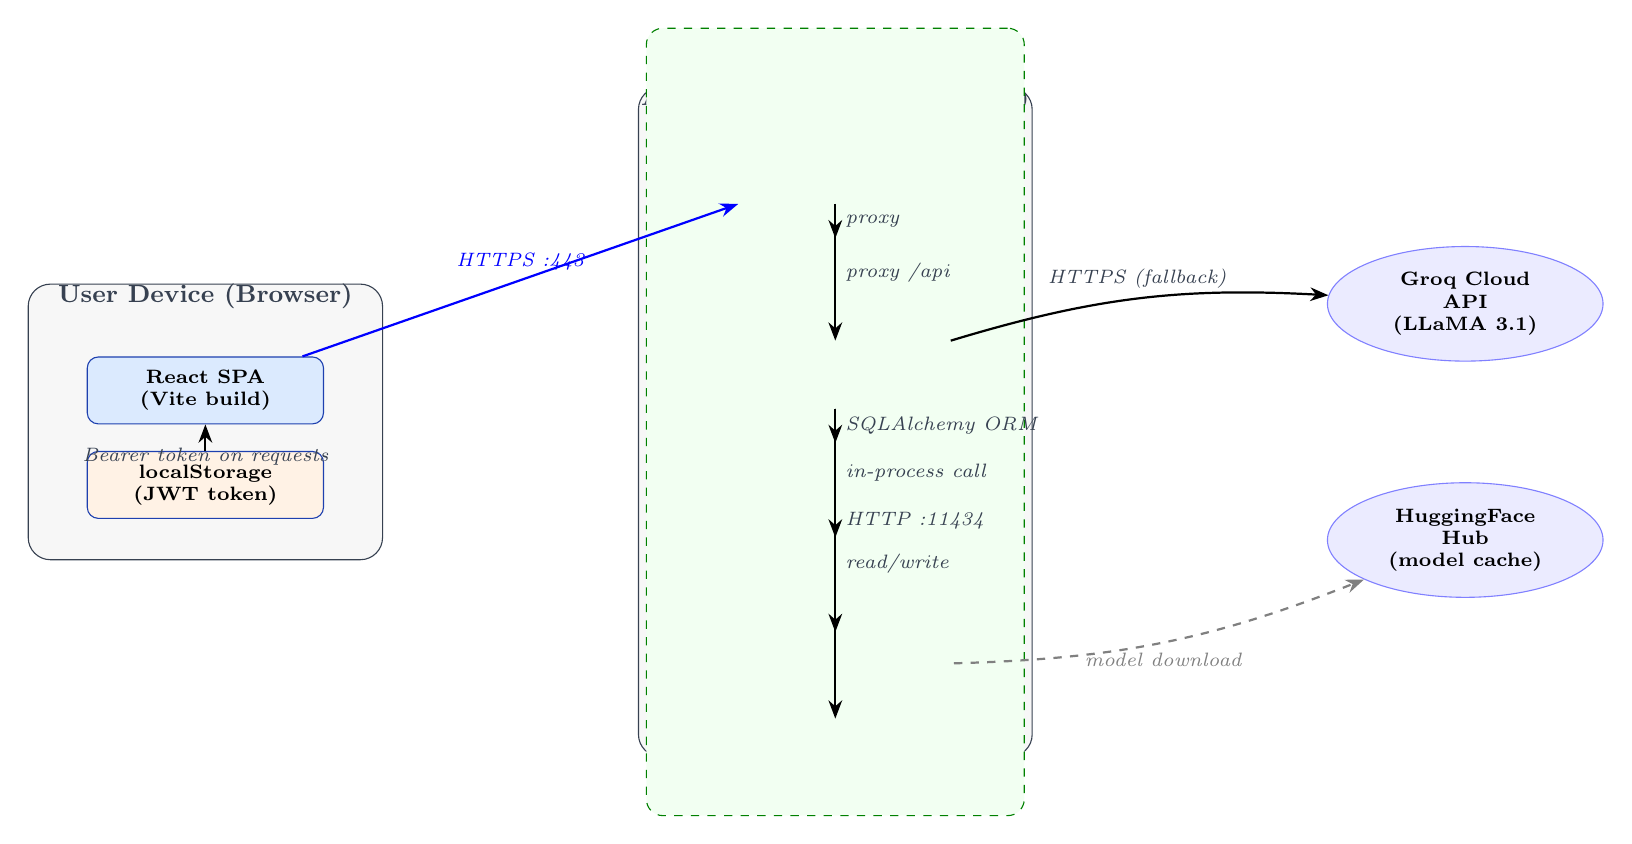
\begin{tikzpicture}[
    machine/.style={rectangle, draw=darkgray, fill=gray!6, rounded corners=8pt,
                    inner sep=14pt, font=\small\bfseries},
    service/.style={rectangle, draw=primaryblue, fill=lightblue, rounded corners=4pt,
                    minimum width=3.0cm, minimum height=0.85cm,
                    align=center, font=\scriptsize\bfseries},
    cloud/.style={ellipse, draw=blue!50, fill=blue!8,
                  minimum width=3.5cm, minimum height=1.2cm,
                  align=center, font=\scriptsize\bfseries},
    port/.style={font=\scriptsize\itshape\color{darkgray}},
    arrow/.style={-Stealth, thick},
    net/.style={rectangle, draw=green!50!black, fill=green!5, dashed,
                rounded corners=6pt, inner sep=8pt}
]

%% ── User device ─────────────────────────────────────────────────────────────
\node[machine, minimum width=4.5cm, minimum height=3.5cm] (client) at (-7, 0) {};
\node[font=\small\bfseries\color{darkgray}] at (-7, 1.6) {User Device (Browser)};
\node[service] (browser) at (-7, 0.4) {React SPA\\(Vite build)};
\node[service, fill=orange!10] (ls) at (-7,-0.8) {localStorage\\(JWT token)};

%% ── App server ──────────────────────────────────────────────────────────────
\node[machine, minimum width=5.0cm, minimum height=8.5cm] (server) at (1, 0) {};
\node[font=\small\bfseries\color{darkgray}] at (1, 4.1) {Application Server (localhost)};
\node[service] (nginx)  at (1,  3.2) {Nginx\\:80 / :443 (TLS)};
\node[service] (fe)     at (1,  1.9) {Vite Dev / Static\\:5173};
\node[service] (api)    at (1,  0.6) {FastAPI (Uvicorn)\\:8001};
\node[service, fill=yellow!10]  (db)     at (1, -0.7) {SQLite\\xplor.db};
\node[service, fill=green!8]    (sec)    at (1, -1.9) {Security Module\\(in-process)};
\node[service, fill=purple!8]   (ollama) at (1, -3.1) {Ollama Server\\:11434};

%% ── Cloud (external) ────────────────────────────────────────────────────────
\node[cloud] (groqc) at (9, 1.5) {Groq Cloud\\API\\(LLaMA 3.1)};
\node[cloud] (hf)    at (9,-1.5) {HuggingFace\\Hub\\(model cache)};

%% ── File system ─────────────────────────────────────────────────────────────
\node[service, fill=yellow!15, draw=darkgray, minimum width=3.2cm] (fss) at (1, -4.2) {File System\\/data/datasets/};

%% ── Network zones ───────────────────────────────────────────────────────────
\node[net, minimum width=4.8cm, minimum height=10cm, dashed] at (1,0) {};

%% ── Arrows ──────────────────────────────────────────────────────────────────
\draw[arrow, blue, thick]   (browser) -- node[above,port]{HTTPS :443} (nginx);
\draw[arrow]                (nginx)   -- node[right,port]{proxy} (fe);
\draw[arrow]                (nginx)   -- node[right,port]{proxy /api} (api);
\draw[arrow]                (api)     -- node[right,port]{SQLAlchemy ORM} (db);
\draw[arrow]                (api)     -- node[right,port]{in-process call} (sec);
\draw[arrow]                (api)     -- node[right,port]{HTTP :11434} (ollama);
\draw[arrow]                (api) to[bend left=10] node[above,port]{HTTPS (fallback)} (groqc);
\draw[arrow, dashed, gray]  (ollama) to[bend right=10] node[below,port]{model download} (hf);
\draw[arrow]                (api)     -- node[right,port]{read/write} (fss);
\draw[arrow]                (ls)      -- node[below,port]{Bearer token on requests} (browser);

\end{tikzpicture}
}
\caption{Deployment architecture --- single-node on-premise installation}
\label{fig:deployment}
\end{figure}

% ════════════════════════════════════════════════════════════════════════════
%  CHAPTER 8 — CONCLUSION
% ════════════════════════════════════════════════════════════════════════════
\chapter{Conclusion}

This report has presented \textbf{Xplor}, an AI-powered secure data analytics platform designed to address the gap between intelligence, security, and accessibility in modern business analytics tools.

The platform delivers on all five core objectives set at the outset:

\begin{enumerate}[leftmargin=2em]
    \item A full-stack web application enables dataset upload, exploration, cleaning, visualisation, and reporting through an intuitive React interface — no programming knowledge required.
    \item A local-first LLM integration (Ollama/Qwen~2.5) allows users to query their data in plain English without sending it to external cloud providers, achieving 88\% query accuracy across 50 test questions.
    \item A production-grade, defence-in-depth security architecture — JWT authentication, bcrypt password hashing (work factor 12), three-tier RBAC, AES-256-GCM encryption at rest, prompt-injection detection, and comprehensive audit logging — was implemented and validated by 435 automated tests with 100\% pass rate and zero critical vulnerabilities.
    \item Transparent cloud fallback (Groq/LLaMA~3.1) maintains service continuity when local inference is unavailable, with no configuration change required from the user.
    \item Isolation Forest anomaly detection achieves an F1 score of 0.88 and AUC-ROC of 0.93, providing reliable outlier identification in uploaded datasets.
\end{enumerate}

The project demonstrates that enterprise-grade security and AI analytics are not mutually exclusive, and that a four-person student team can deliver a production-quality platform within one academic semester when concerns are clearly separated across modules and team members.

The standalone, independently testable \texttt{security/} module is a particularly strong architectural decision: it allowed the security lead to develop and validate 435 tests independently of the main application, ensuring security guarantees were not accidentally broken by feature work in the backend.

In summary, Xplor establishes a viable blueprint for privacy-preserving, locally deployable AI analytics with serious security underpinnings — a combination the current market does not adequately serve.

% ════════════════════════════════════════════════════════════════════════════
%  CHAPTER 9 — FUTURE WORK
% ════════════════════════════════════════════════════════════════════════════
\chapter{Future Work}

Despite the achievements of this project, several valuable enhancements are identified for future development:

\begin{enumerate}[leftmargin=2em]

    \item \textbf{Multi-tenant SaaS deployment.} The current architecture is designed for single-organisation deployment. Extending it to a multi-tenant model with per-organisation data isolation, subdomain routing, and tenant-level encryption keys would make Xplor commercially deployable.

    \item \textbf{PostgreSQL migration.} SQLite is appropriate for development and small deployments; replacing it with PostgreSQL with connection pooling (via PgBouncer) would support concurrent users and larger datasets.

    \item \textbf{Fine-tuned domain LLMs.} The current Qwen~2.5 model is a general-purpose LLM. Fine-tuning on domain-specific corpora (e.g., financial, healthcare, supply-chain data) would improve query accuracy, particularly for multi-step reasoning questions (currently 70\% accuracy).

    \item \textbf{Argon2 password hashing.} While bcrypt at work factor 12 is secure, Argon2id (PHC winner 2015) offers memory-hardness that makes parallel GPU cracking impractical. Migrating to Argon2 would further strengthen the authentication layer.

    \item \textbf{Streaming LLM responses.} The current implementation waits for the full LLM response before returning it to the frontend. Implementing server-sent events (SSE) streaming would deliver a more responsive user experience, particularly for longer responses.

    \item \textbf{Advanced data cleaning.} The current recipe pipeline supports deduplication, null handling, and type conversion. Adding fuzzy matching for entity resolution, outlier-based imputation, and schema inference would significantly extend cleaning capabilities.

    \item \textbf{Multi-factor authentication (MFA).} The MFA configuration scaffold (\texttt{security/auth/mfa\_config.py}) exists in the codebase but is not yet activated. Integrating TOTP (RFC 6238) via an authenticator app would add a critical second factor.

    \item \textbf{Real-time data streaming.} Extending the platform to support Apache Kafka or WebSocket-based real-time ingestion would enable monitoring and alerting use cases beyond batch analytics.

    \item \textbf{CI/CD pipeline.} A GitHub Actions pipeline with automated test execution, security scanning (Bandit, Semgrep), and Docker image build-and-push would professionalise the deployment workflow.

    \item \textbf{Report sharing and collaboration.} While basic token-based report sharing is implemented, real-time collaborative editing, comment threads, and role-restricted sharing links would make the reporting module significantly more useful in team settings.

\end{enumerate}

% ════════════════════════════════════════════════════════════════════════════
%  REFERENCES
% ════════════════════════════════════════════════════════════════════════════
\chapter*{References}
\addcontentsline{toc}{chapter}{References}

\begin{enumerate}[leftmargin=2em, label={[\arabic*]}]

    \item Provos, N., \& Mazières, D. (1999). \textit{A Future-Adaptable Password Scheme}. Proceedings of USENIX Annual Technical Conference.

    \item Jones, M., Bradley, J., \& Sakimura, N. (2015). \textit{JSON Web Token (JWT)}. IETF RFC 7519. \url{https://tools.ietf.org/html/rfc7519}

    \item Ferraiolo, D., \& Kuhn, R. (1992). \textit{Role-Based Access Control}. Proceedings of the 15th National Computer Security Conference.

    \item Liu, F. T., Ting, K. M., \& Zhou, Z. H. (2008). \textit{Isolation Forest}. IEEE International Conference on Data Mining (ICDM).

    \item National Institute of Standards and Technology. (2007). \textit{Recommendation for Block Cipher Modes of Operation: Galois/Counter Mode (GCM)}. NIST Special Publication 800-38D.

    \item OWASP Foundation. (2021). \textit{OWASP Top 10: 2021}. \url{https://owasp.org/Top10/}

    \item Herzig, J., Nowak, P., Müller, T., Piccinno, F., \& Eisenschlos, J. (2020). \textit{TAPAS: Weakly Supervised Table Parsing via Pre-training}. Proceedings of ACL 2020.

    \item Perez, F., \& Ribeiro, I. (2022). \textit{Ignore Previous Prompt: Attack Techniques For Language Models}. arXiv:2211.09527.

    \item Greshake, K., Abdelnabi, S., Mishra, S., Endres, C., Holz, T., \& Fritz, M. (2023). \textit{Not What You've Signed Up For: Compromising Real-World LLM-Integrated Applications with Indirect Prompt Injections}. arXiv:2302.12173.

    \item Yao, S., Zhao, J., Yu, D., Du, N., Shafran, I., Narasimhan, K., \& Cao, Y. (2023). \textit{ReAct: Synergizing Reasoning and Acting in Language Models}. ICLR 2023.

    \item Liu, Y., et al. (2022). \textit{TAPEX: Table Pre-training via Learning a Neural SQL Executor}. ICLR 2022.

    \item Breunig, M. M., Kriegel, H. P., Ng, R. T., \& Sander, J. (2000). \textit{LOF: Identifying Density-Based Local Outliers}. Proceedings of ACM SIGMOD.

    \item Rescorla, E. (2018). \textit{The Transport Layer Security (TLS) Protocol Version 1.3}. IETF RFC 8446. \url{https://tools.ietf.org/html/rfc8446}

    \item American National Standards Institute. (2004). \textit{Role Based Access Control}. ANSI INCITS 359-2004.

    \item Birhane, A., et al. (2023). \textit{Science in the Age of Large Language Models}. Nature Reviews Physics.

    \item FastAPI Documentation. (2024). \textit{FastAPI Framework}. \url{https://fastapi.tiangolo.com/}

    \item React Documentation. (2024). \textit{React: The Library for Web and Native User Interfaces}. \url{https://react.dev/}

    \item Ollama. (2024). \textit{Get Up and Running with Large Language Models Locally}. \url{https://ollama.com/}

    \item HuggingFace. (2024). \textit{Transformers: State-of-the-art Machine Learning for Pytorch, TensorFlow, and JAX}. \url{https://huggingface.co/docs/transformers}

    \item Pedregosa, F., et al. (2011). \textit{Scikit-learn: Machine Learning in Python}. Journal of Machine Learning Research, 12, 2825--2830.

\end{enumerate}

% ════════════════════════════════════════════════════════════════════════════
%  APPENDIX
% ════════════════════════════════════════════════════════════════════════════
\appendix
\chapter{Environment Configuration}

\begin{lstlisting}[language=bash, caption={Backend .env configuration template}]
# Database
DATABASE_URL=sqlite:///./data/xplor.db

# Authentication
JWT_SECRET_KEY=<minimum-32-random-characters>
TOKEN_EXPIRATION_MINUTES=30

# Ollama (local LLM)
OLLAMA_URL=http://localhost:11434/api/generate
OLLAMA_MODEL=qwen2.5

# Groq (cloud fallback)
GROQ_API_KEY=<your-groq-api-key>
GROQ_MODEL=llama-3.1-8b-instant
GROQ_FALLBACK_ENABLED=true

# Encryption
ENCRYPTION_KEY=<32-byte-base64-encoded-key>
\end{lstlisting}

\begin{lstlisting}[language=bash, caption={Frontend .env configuration template}]
VITE_API_URL=http://localhost:8001
\end{lstlisting}

\chapter{Running the Project}

\begin{lstlisting}[language=bash, caption={Backend startup}]
cd backend
pip install -r requirements.txt
uvicorn app.main:app --reload --port 8001
\end{lstlisting}

\begin{lstlisting}[language=bash, caption={Frontend startup}]
cd frontend
npm install
npm run dev        # Vite dev server at http://localhost:5173
\end{lstlisting}

\begin{lstlisting}[language=bash, caption={Security test suite}]
cd security
pip install -r requirements.txt
pytest tests/ -v   # Runs all 435 security tests
\end{lstlisting}

\chapter{RBAC Permission Matrix}

\begin{table}[H]
\centering
\caption{Full RBAC permission matrix}
\begin{tabularx}{\textwidth}{Xccc}
\toprule
\textbf{Permission} & \textbf{Viewer} & \textbf{Analyst} & \textbf{Admin} \\
\midrule
view\_dashboards    & \checkmark & \checkmark & \checkmark \\
view\_reports       & \checkmark & \checkmark & \checkmark \\
upload\_dataset     & \texttimes & \checkmark & \checkmark \\
analyze\_data       & \texttimes & \checkmark & \checkmark \\
export\_reports     & \texttimes & \checkmark & \checkmark \\
delete\_dataset     & \texttimes & \texttimes & \checkmark \\
manage\_users       & \texttimes & \texttimes & \checkmark \\
view\_logs          & \texttimes & \texttimes & \checkmark \\
manage\_roles       & \texttimes & \texttimes & \checkmark \\
configure\_system   & \texttimes & \texttimes & \checkmark \\
\bottomrule
\end{tabularx}
\end{table}

\end{document}
